\chapter{Detailed Attempt Log}

This appendix records the detailed experimental sequence used to build the
final thesis narrative. It is intentionally more operational than the main
chapters: the purpose is to show how the final design emerged from earlier
failures, not to re-argue every result.

\section{Early image-to-image phase}

The first implementation treated CKM prediction as an aligned
image-to-image translation problem. This was a reasonable starting point
because the inputs and outputs share the same \(513\times513\) grid. A U-Net
generator produced dense maps and a PatchGAN discriminator judged local
patches. The problem was objective mismatch. A propagation map is not a
natural image: a visually plausible texture can be numerically wrong by many
decibels. This is why later attempts reduced or removed adversarial pressure
and moved toward explicit regression losses.

In hindsight, the cGAN branch was useful because it made this mismatch visible
early. The discriminator rewarded local realism, but the thesis metric rewards
calibrated physical values under a ground mask. A sharp NLoS-looking shadow
that is \SI{30}{dB} too low is still a bad radio map. This is why the later
work stopped treating texture quality as a proxy for propagation quality and
started reporting LoS/NLoS, topology, and antenna-height errors separately.

Tries 9--14 introduced height conditioning and LoS/NLoS-aware evaluation.
These changes were not cosmetic. UAV height changes the path-length geometry
and therefore cannot be hidden in the sample index. Likewise, LoS and NLoS
pixels follow different propagation laws, so mixing them into one global score
made diagnosis difficult.

\section{Artifact removal and masked supervision}

Tries 15--22 attacked three visible problems: checkerboard artifacts, loss of
thin street and edge structure, and weak radial consistency. GroupNorm replaced
BatchNorm because the full-resolution jobs used very small batches. A distance
channel exposed the most important geometric variable directly. Try 20 isolated
the bilinear decoder change, Try 21 isolated multiscale supervision, and Try
22 combined both. In the early contract, Try 22 was the strongest clean
path-loss baseline at about \SI{16.72}{dB}.

The next methodological correction was more important than another decoder
change: pixels inside buildings are not valid receiver locations. After Try
33, the project excluded \(topology\_map \ne 0\) pixels from the loss, from
validation and test metrics, and from error-map visualization. This made the
task stricter and invalidated easy comparisons to older runs that had not used
the same mask.

\section{Prior-guided residual phase}

Try 41 made the residual formulation explicit:
\[
  \widehat{\mathrm{PL}} =
  \mathrm{PL}_{\mathrm{prior}} + r_\theta(x).
\]
The initial raw formula prior was poor, with validation RMSE around
\SI{67.23}{dB}. Train-only regime-aware calibration improved it to about
\SI{24.16}{dB}. This result was simultaneously encouraging and limiting:
the prior clearly contained useful information, but it was not enough to
replace learning.

Try 42 moved away from the old U-Net/cGAN family toward a PMNet-style residual
regressor. Try 49 added prior-confidence logic and robust loss weighting; its
stage-1 branch reached about \SI{18.87}{dB}, while the calibrated prior stayed
near \SI{23.57}{dB}. The main failure mode was a heavy tail: many pixels were
moderately accurate, but some NLoS pixels produced very large errors, so RMSE
stayed much larger than MAE.

The PMNet control line also clarified what the prior was and was not doing.
Try 44, a no-prior PMNet-v3-style control, learned the LoS part to roughly
\SI{4.27}{dB} but still left NLoS near \SI{38.58}{dB}. That result is important
because it cannot be blamed on a bad physical-prior channel. The model had
enough information to recover the smooth radial component, but not enough
distributional structure to place blocked-link values reliably.

Try 48 and Try 50 were useful negative evidence. Several richer NLoS priors
and structural prior variants were tested, but a candidate refined prior at
\SI{24.1777}{dB} did not beat the older \SI{23.5746}{dB} calibration, and the
best Try 50 NLoS sandbox still remained near \SI{41}{dB}. The conclusion was
that NLoS required more than a scalar correction over a LoS-shaped prior.

\section{Final distribution and prior phase}

Try 66 consolidated the PMHHNet family: physical channels, GroupNorm, height
FiLM, and expert routing. It reached \SI{9.41}{dB} overall, but the split
metric showed the deeper issue: \SI{3.75}{dB} LoS and \SI{31.48}{dB} NLoS.
The project was no longer failing uniformly.

Several PMHHNet-era fixes were real engineering improvements, but none changed
the basic diagnosis by themselves. Disabling an overly tolerant Huber setup,
restoring full-resolution reconstruction losses, reducing excessive
regularisation, removing centre-heavy corridor weighting, and restoring early
high-frequency injection all made training more honest. Yet the no-prior
reruns still showed the same pattern: LoS became reasonable, while NLoS
remained much worse. The bottleneck had moved from backbone design to target
modelling.

Try 76 reframed NLoS as a distributional problem. Instead of predicting a
single value everywhere, the model predicted sample-level mixture structure
and then placed components spatially. This produced a much stronger NLoS path
loss result, around \SI{3.34}{dB} pixel-weighted in the DirectML summary.
The key lesson was that the prior was not the only route to a good model. If a
network can estimate the correct marginal distribution and assign pixels to
its components, it can approach the performance of a strong prior even without
being handed the prior explicitly.

Try 78 then showed that LoS path loss was even more deterministic than the
neural history suggested. The dominant residual over FSPL was a ring field,
well explained by the enhanced two-ray model with fitted effective
reflection parameters. Try 79 applied a related philosophy to delay and
angular spreads: use log-domain, regime-wise calibration over geometry and
local morphology features. Try 80 is the synthesis: frozen Try 78/79 priors
plus a neural model that predicts bounded residuals.

The final spread attempts added one more lesson: path loss, delay spread, and
angular spread should not be forced into the same mental template. Path-loss
LoS is structured and almost deterministic; path-loss NLoS is narrow in value
but noisy in spatial placement. Delay and angular spread are different again:
their most informative behaviour is often in NLoS, where multipath and
scattering create the tail that matters for channel quality. This is why the
final attempt history ends with distributions and regime-aware targets rather
than only with larger encoders.

\chapter{Try 80 Configuration Summary}

The active Try 80 configuration uses the canonical dataset
\texttt{CKM\_Dataset\_270326.h5}, image size \(513\times513\), split seed 42,
and validation/test ratios of 15\% each after city assignment. It uses
precomputed priors when available through
\texttt{try80\_precomputed\_priors.h5}, but the priors are deterministic and
can also be recomputed.

\begin{table}[ht]
\centering
\caption{Main Try 80 configuration values.}
\label{tab:try80_config_appendix}
\begin{tabularx}{\textwidth}{lX}
\toprule
Category & Value \\
\midrule
Input channels & 9: topology, LoS mask, NLoS mask, ground mask, combined
path-loss prior, LoS path-loss prior, NLoS path-loss prior, delay-spread prior,
angular-spread prior. \\
Height conditioning & Sinusoidal embedding with FiLM modulation. \\
Backbone & Four-scale GroupNorm encoder-decoder, base width 96. \\
Residual distribution & Three mixture components per task/region head. \\
Residual limits & Path loss: 2 dB LoS and 4 dB NLoS; delay spread: 30 ns LoS
and 40 ns NLoS; angular spread: 9 degrees LoS and 13 degrees NLoS. \\
Main losses & Map NLL, distribution KL, moment matching, anchor,
prior-guard, outlier budget, RMSE, and MAE. \\
Training & AdamW, learning rate \(2\times10^{-4}\), weight decay 0.01,
120 epochs, batch size 1, gradient accumulation 8. \\
\bottomrule
\end{tabularx}
\end{table}

The final prediction for each task \(t\) has the same conceptual form:
\[
  \hat y_t(x) = y_{t,\mathrm{prior}}(x) + \alpha_t(x)\Delta_t(x),
  \qquad 0 \le \alpha_t(x) \le 1.
\]
This is the central safety mechanism. The network is allowed to improve the
prior, but the residual is bounded and gated. The prior-guard term then
penalizes cases where the model moves away from the prior and becomes worse.

\chapter{Formula Placement}

The appendix is kept as an audit trail, not as a second methodology chapter.
Detailed formulas are therefore placed where they are first used in the main
technical narrative. This avoids having two slightly different versions of the
same prior definition.

\begin{table}[ht]
\centering
\caption{Location of the main mathematical definitions.}
\label{tab:formula_location_appendix}
\begin{tabularx}{\textwidth}{lX}
\toprule
Topic & Location in the main text \\
\midrule
Ground-pixel mask and RMSE contract &
Chapter~3, Eqs.~\ref{eq:ground_mask}--\ref{eq:rmse}. \\
Residual-learning formulation &
Chapter~3, Eq.~\ref{eq:prior_residual}. \\
Height conditioning and FiLM modulation &
Chapter~3, Eqs.~\ref{eq:sin_film}--\ref{eq:film_math}. \\
Try 78 LoS path-loss prior &
Section~\ref{sec:try78_detail}, especially Eqs.~\ref{eq:fspl},
\ref{eq:field_sum}, \ref{eq:c2ray}, and \ref{eq:pl_los}. \\
Try 78 NLoS calibration &
Section~\ref{sec:nlos_branch}, especially Eqs.~\ref{eq:cost231},
\ref{eq:a2g_nlos}, \ref{eq:x78}, and \ref{eq:pl_nlos_final}. \\
Try 79 spread priors &
Section~\ref{sec:try79_detail}, especially Eqs.~\ref{eq:raw_spread},
\ref{eq:x79}, \ref{eq:ridge}, and \ref{eq:inv_log}. \\
Try 80 prior-anchored GMM &
Section~\ref{sec:try80_detail}, especially Eqs.~\ref{eq:try80_mu},
\ref{eq:try80_point}, and \ref{eq:try80_loss}. \\
\bottomrule
\end{tabularx}
\end{table}

This placement makes the appendix optional for understanding the mathematics.
A reader can follow the thesis from the main chapters alone; the appendix adds
the chronological and reproducibility context behind those choices.

\chapter{Representative Try 80 Inspection Panels}

The qualitative appendix is generated with
\texttt{TFGpractice/TFGEightiethTry80/scripts/}\newline
\texttt{generate\_try80\_appendix\_panels.py}. It uses the validation split,
the near-final huge path-loss-finetuned checkpoint, DirectML inference, and
the frozen Try 78/79 priors. The script selects one validation
sample for each macro expert
\((\mathrm{open},\mathrm{mixed},\mathrm{dense})\times
(\mathrm{low},\mathrm{mid},\mathrm{high})\). It keeps candidates for which
Try 80 beats the frozen prior on all three outputs, then chooses the
best-mean-RMSE candidate while drawing from different cities where the
validation split provides visually distinct examples. The manifest next to
the images records filenames, city, sample, antenna height, and per-task RMSE.

The script can emit both a wide and a tall layout, but the thesis keeps only
the tall \(6\times 3\) version to avoid duplicating the same evidence. In this
layout, the six inspection stages are rows and the three targets are columns.
The six inspection stages, in order, are:

\begin{enumerate}
\setlength\itemsep{0.15em}
  \item \textbf{Ground truth} --- the ray-traced reference field.
  \item \textbf{Frozen prior (Try 78/79)} --- the calibrated analytic prior
        that Try 80 receives as an input channel and anchors to.
  \item \textbf{Try 80 prediction} --- the final residual-over-prior output
        of the joint model, in the same colour scale as columns 1--2.
  \item \textbf{Context} --- topology height for the path-loss row, NLoS
        support for the delay-spread row, and LoS support for the
        angular-spread row.
  \item \textbf{Prior error} --- the signed difference
        \(\mathrm{Prior}-\mathrm{GT}\). Red indicates a prior overshoot,
        blue indicates a prior undershoot, and white indicates where the
        analytic prior is already accurate.
  \item \textbf{Model correction} --- the signed residual
        \(\mathrm{Try\,80}-\mathrm{Prior}\) that the neural head applies on
        top of the prior. If the model has learned a useful residual,
        row~6 should \emph{anti-correlate} with row~5: where the prior
        is too high, the model should push down, and vice versa.
\end{enumerate}

Rows 5 and 6 are therefore the main \emph{diagnostic} rows: the thesis
claim is that Try 80 is a prior-anchored residual corrector, and the visible
agreement (in sign and location) between the prior-error map and the
model-correction map is the direct qualitative evidence for that claim.

\begin{table}[H]
\centering
\caption{Try 80 appendix panels generated from validation samples with the
near-final huge checkpoint.}
\label{tab:try80_appendix_panels}
\footnotesize
\begin{tabular}{llll}
\toprule
Expert & City & Sample & Height bin \\
\midrule
open/low & Segovia & sample\_13213 & low \\
open/mid & Segovia & sample\_13215 & mid \\
open/high & Nazareth & sample\_10722 & high \\
mixed/low & Dubrovnik & sample\_05288 & low \\
mixed/mid & Nice & sample\_10828 & mid \\
mixed/high & Nice & sample\_10814 & high \\
dense/low & Chiang Mai & sample\_04519 & low \\
dense/mid & Tunis & sample\_14651 & mid \\
dense/high & Tunis & sample\_14694 & high \\
\bottomrule
\end{tabular}
\end{table}

The exact PNG filenames and per-sample RMSE values are stored in
\newline
\texttt{img/thesis\_figures/try80\_appendix\_panels/manifest.json}.

\clearpage
\begin{figure}[p]
\centering
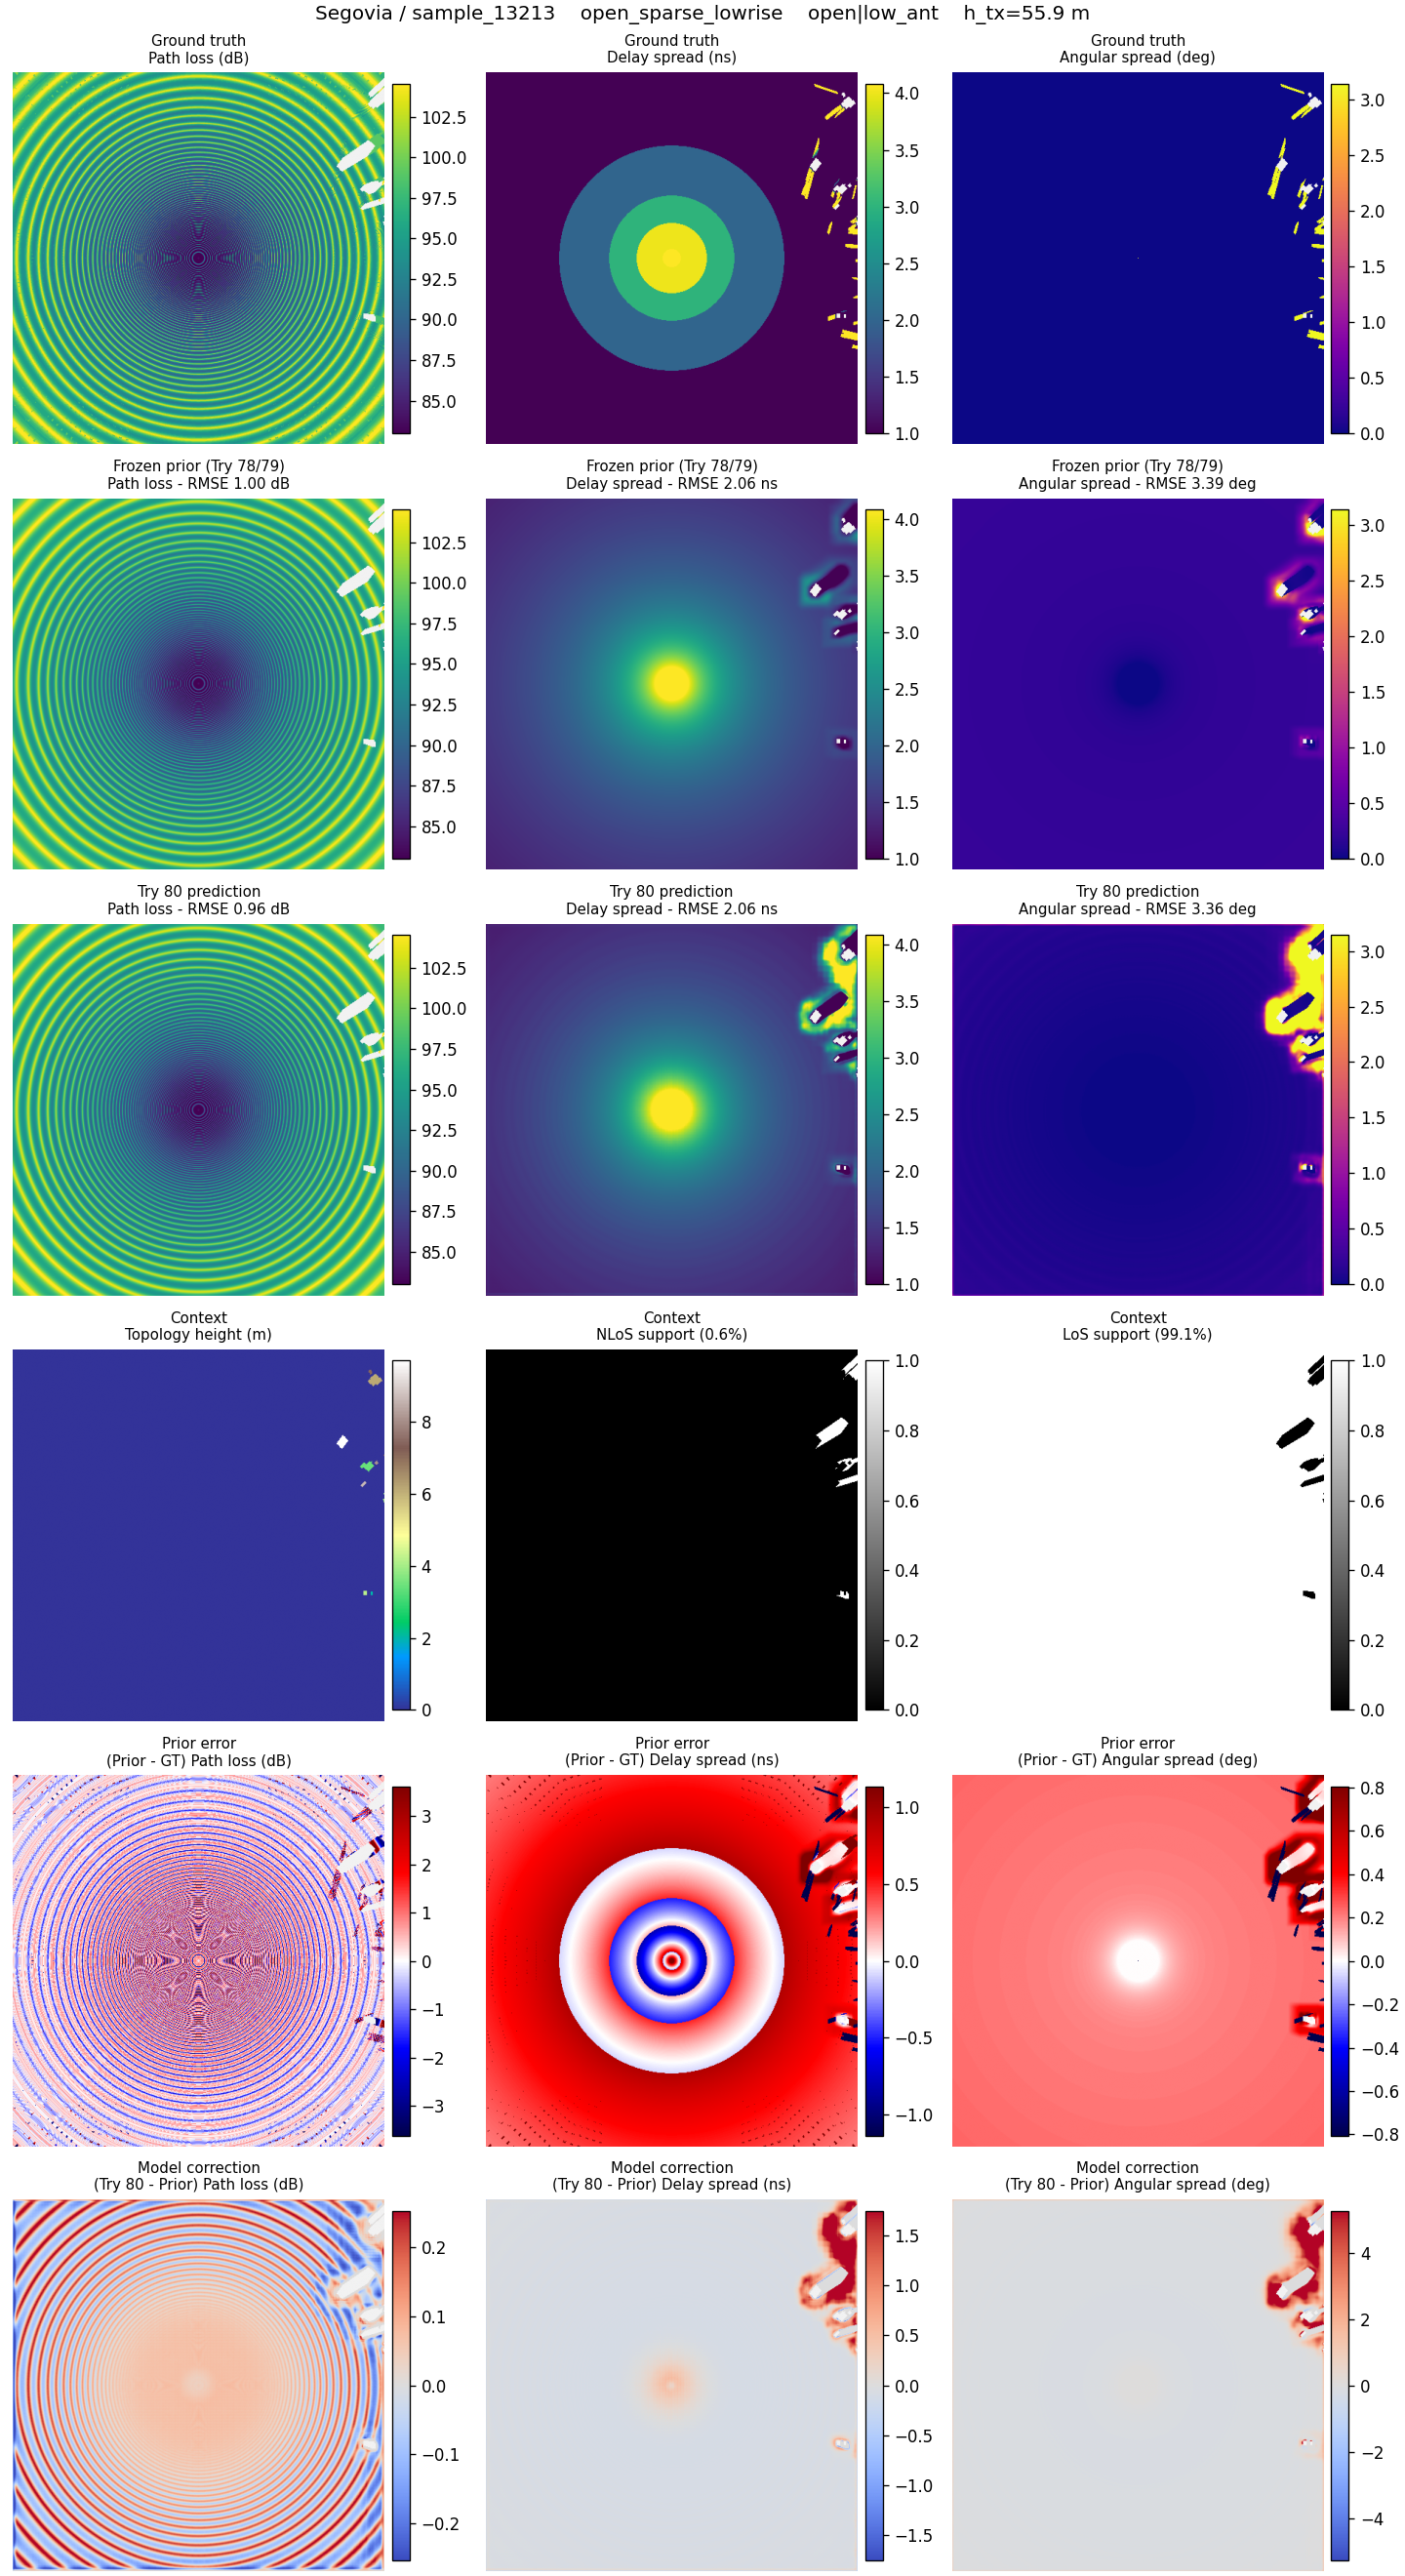
\includegraphics[width=\textwidth,height=0.88\textheight,keepaspectratio]{img/thesis_figures/try80_appendix_panels/try80_panel_open_low_ant_Segovia_sample_13213_6x3.png}
\caption{Try 80 \(6\times3\) inspection panel for an open, low-antenna
validation sample in Segovia.}
\label{fig:appendix_try80_open_low}
\end{figure}

\clearpage
\begin{figure}[p]
\centering
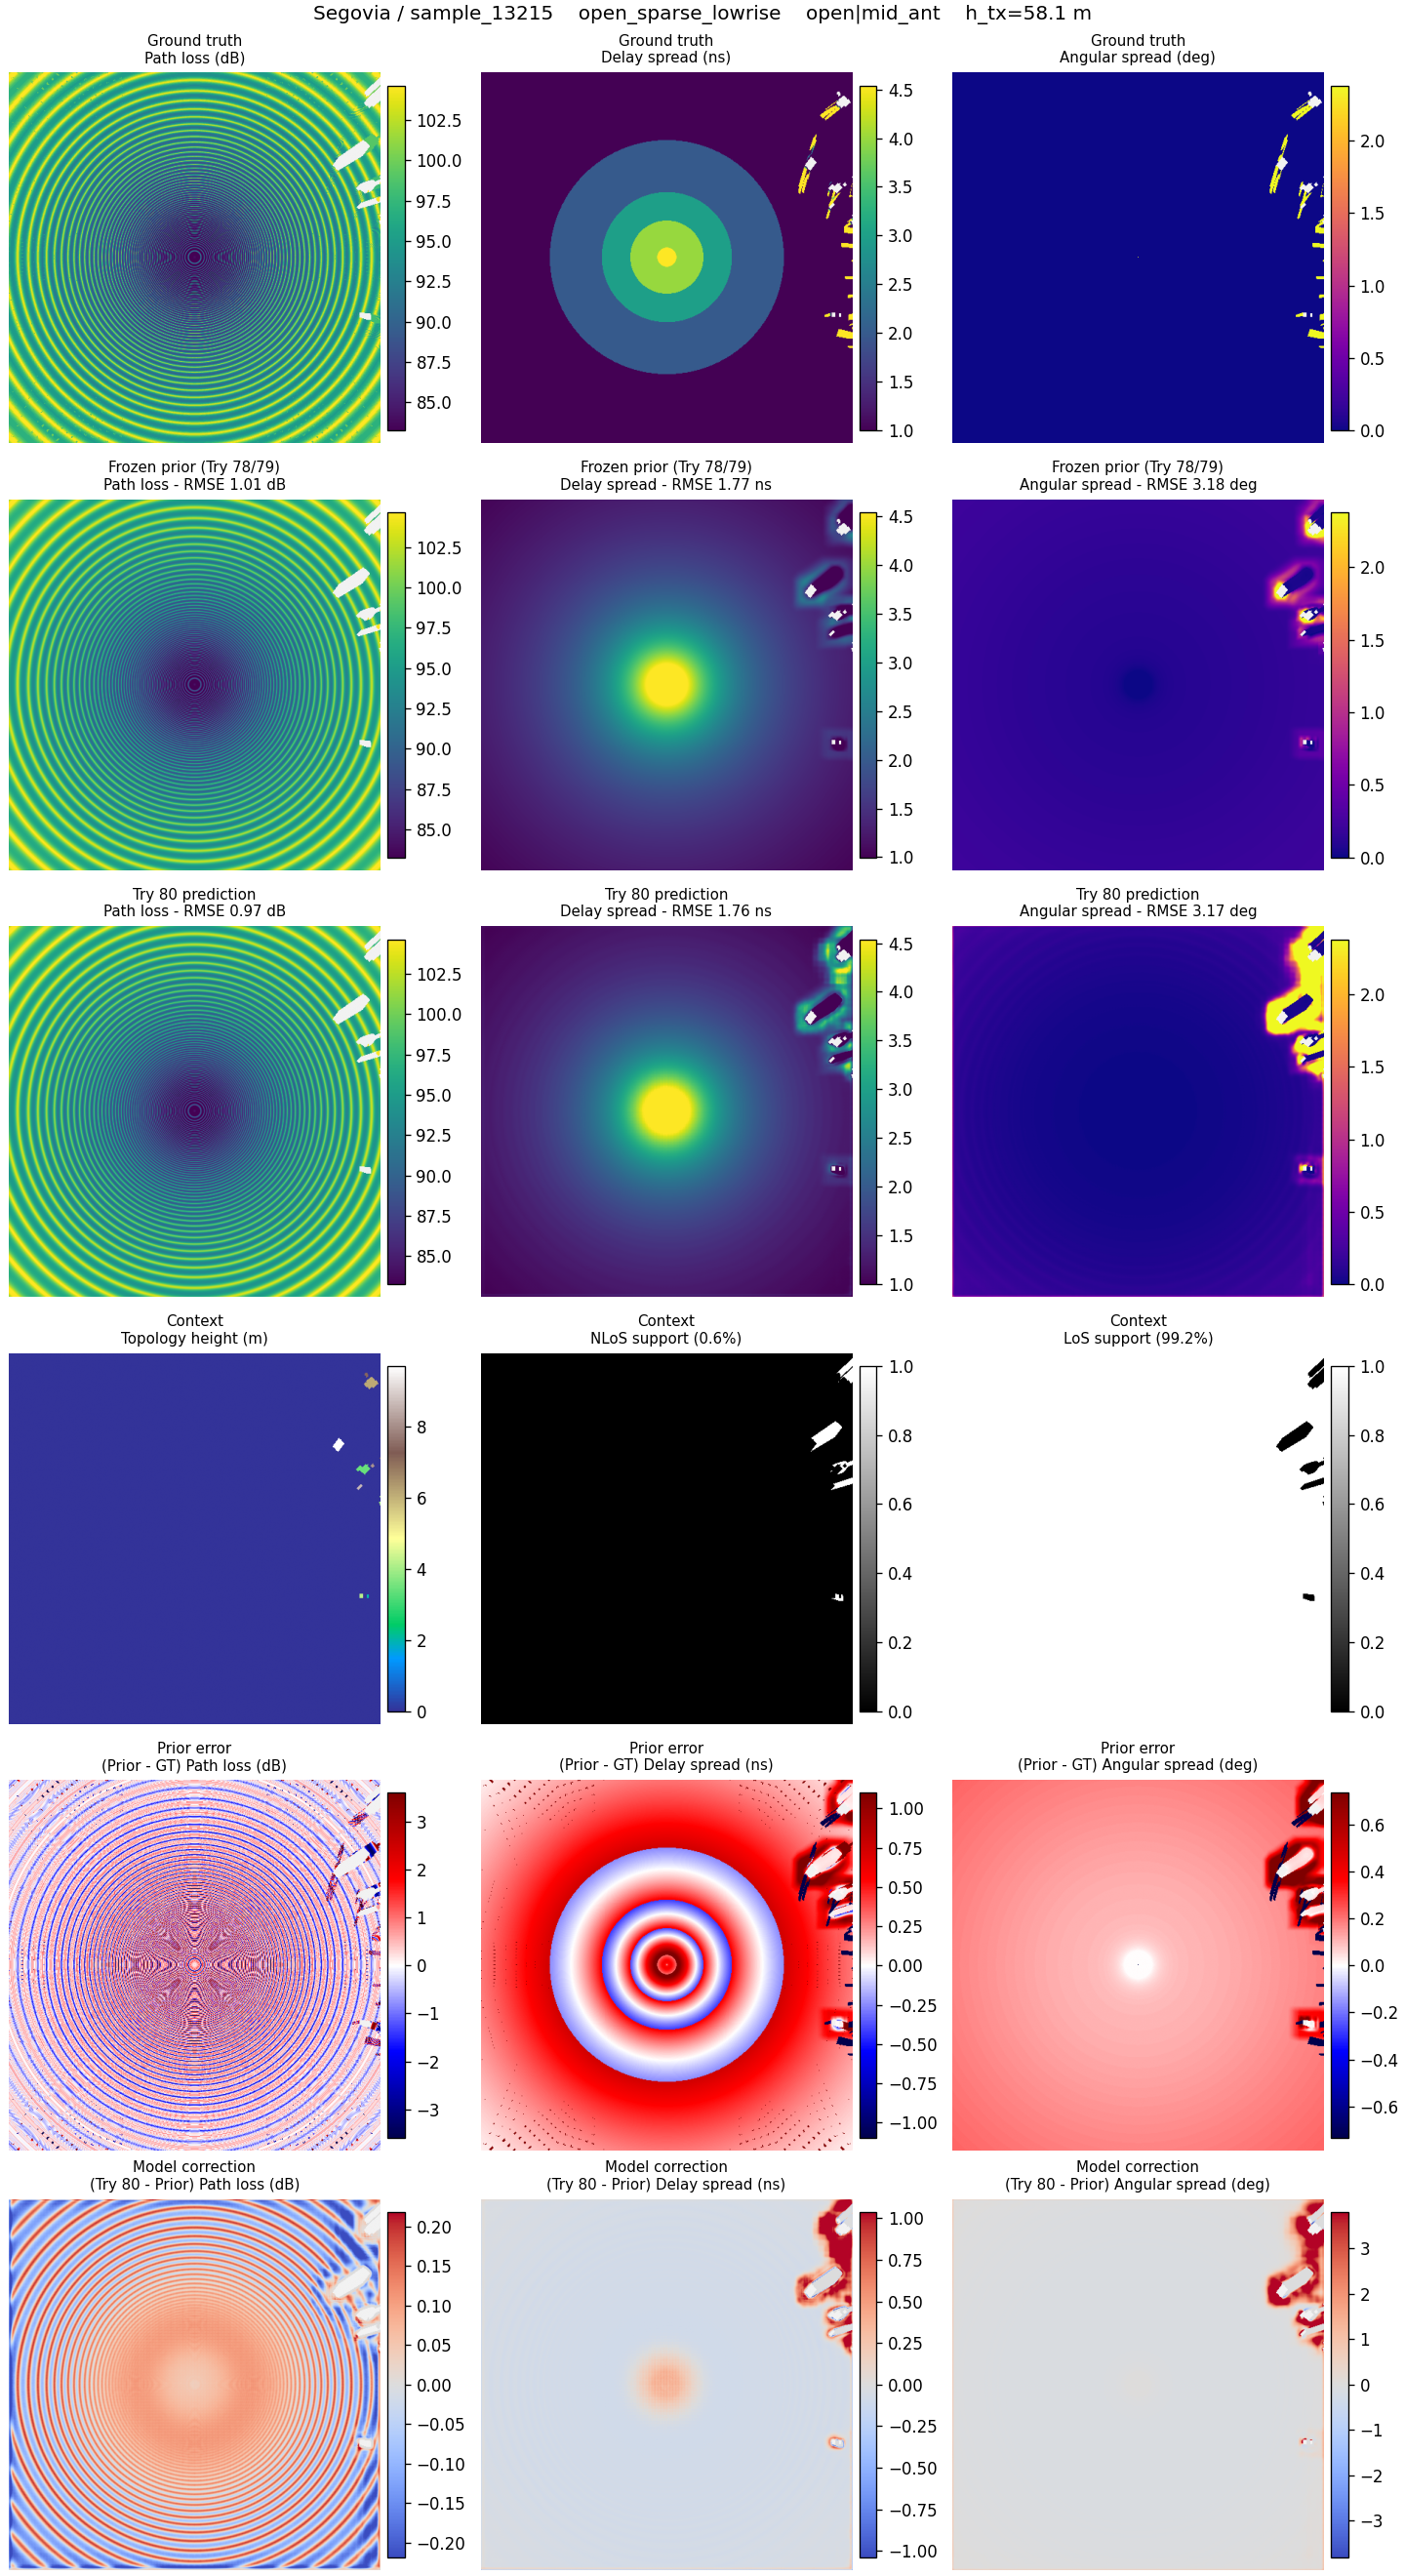
\includegraphics[width=\textwidth,height=0.88\textheight,keepaspectratio]{img/thesis_figures/try80_appendix_panels/try80_panel_open_mid_ant_Segovia_sample_13215_6x3.png}
\caption{Try 80 \(6\times3\) inspection panel for an open, mid-antenna
validation sample in Segovia.}
\label{fig:appendix_try80_open_mid}
\end{figure}

\clearpage
\begin{figure}[p]
\centering
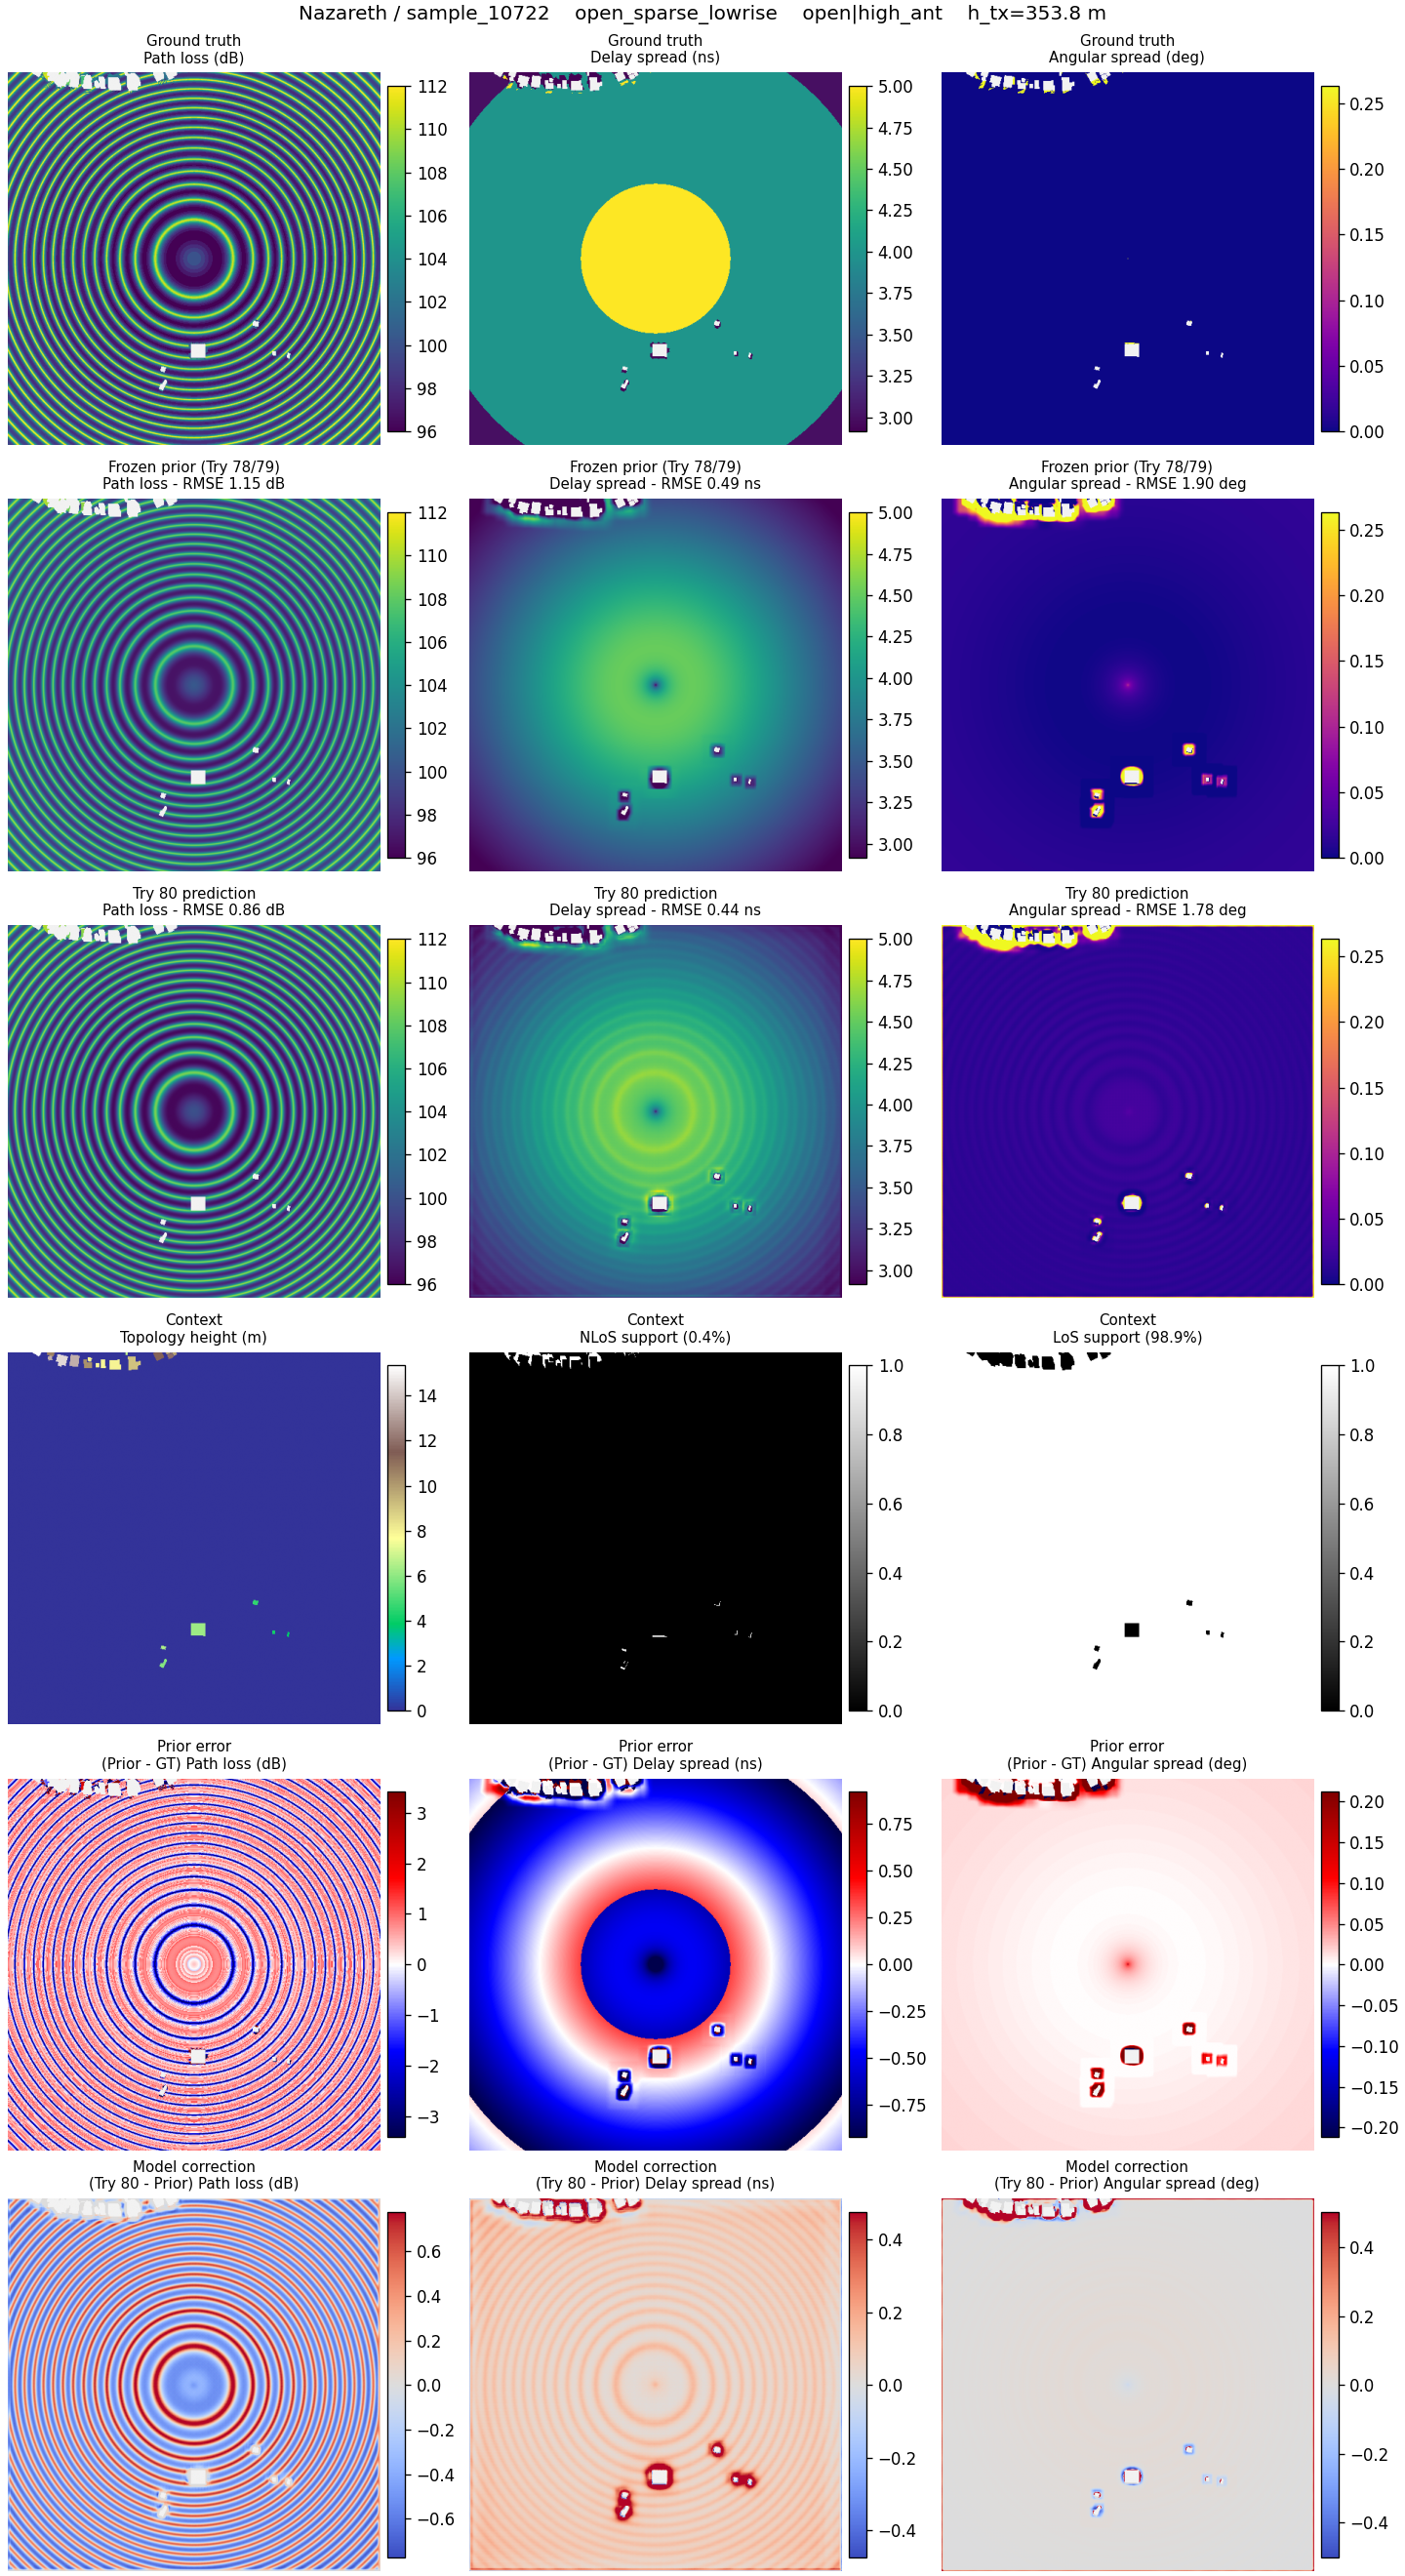
\includegraphics[width=\textwidth,height=0.88\textheight,keepaspectratio]{img/thesis_figures/try80_appendix_panels/try80_panel_open_high_ant_Nazareth_sample_10722_6x3.png}
\caption{Try 80 \(6\times3\) inspection panel for an open, high-antenna
validation sample in Nazareth.}
\label{fig:appendix_try80_open_high}
\end{figure}

\clearpage
\begin{figure}[p]
\centering
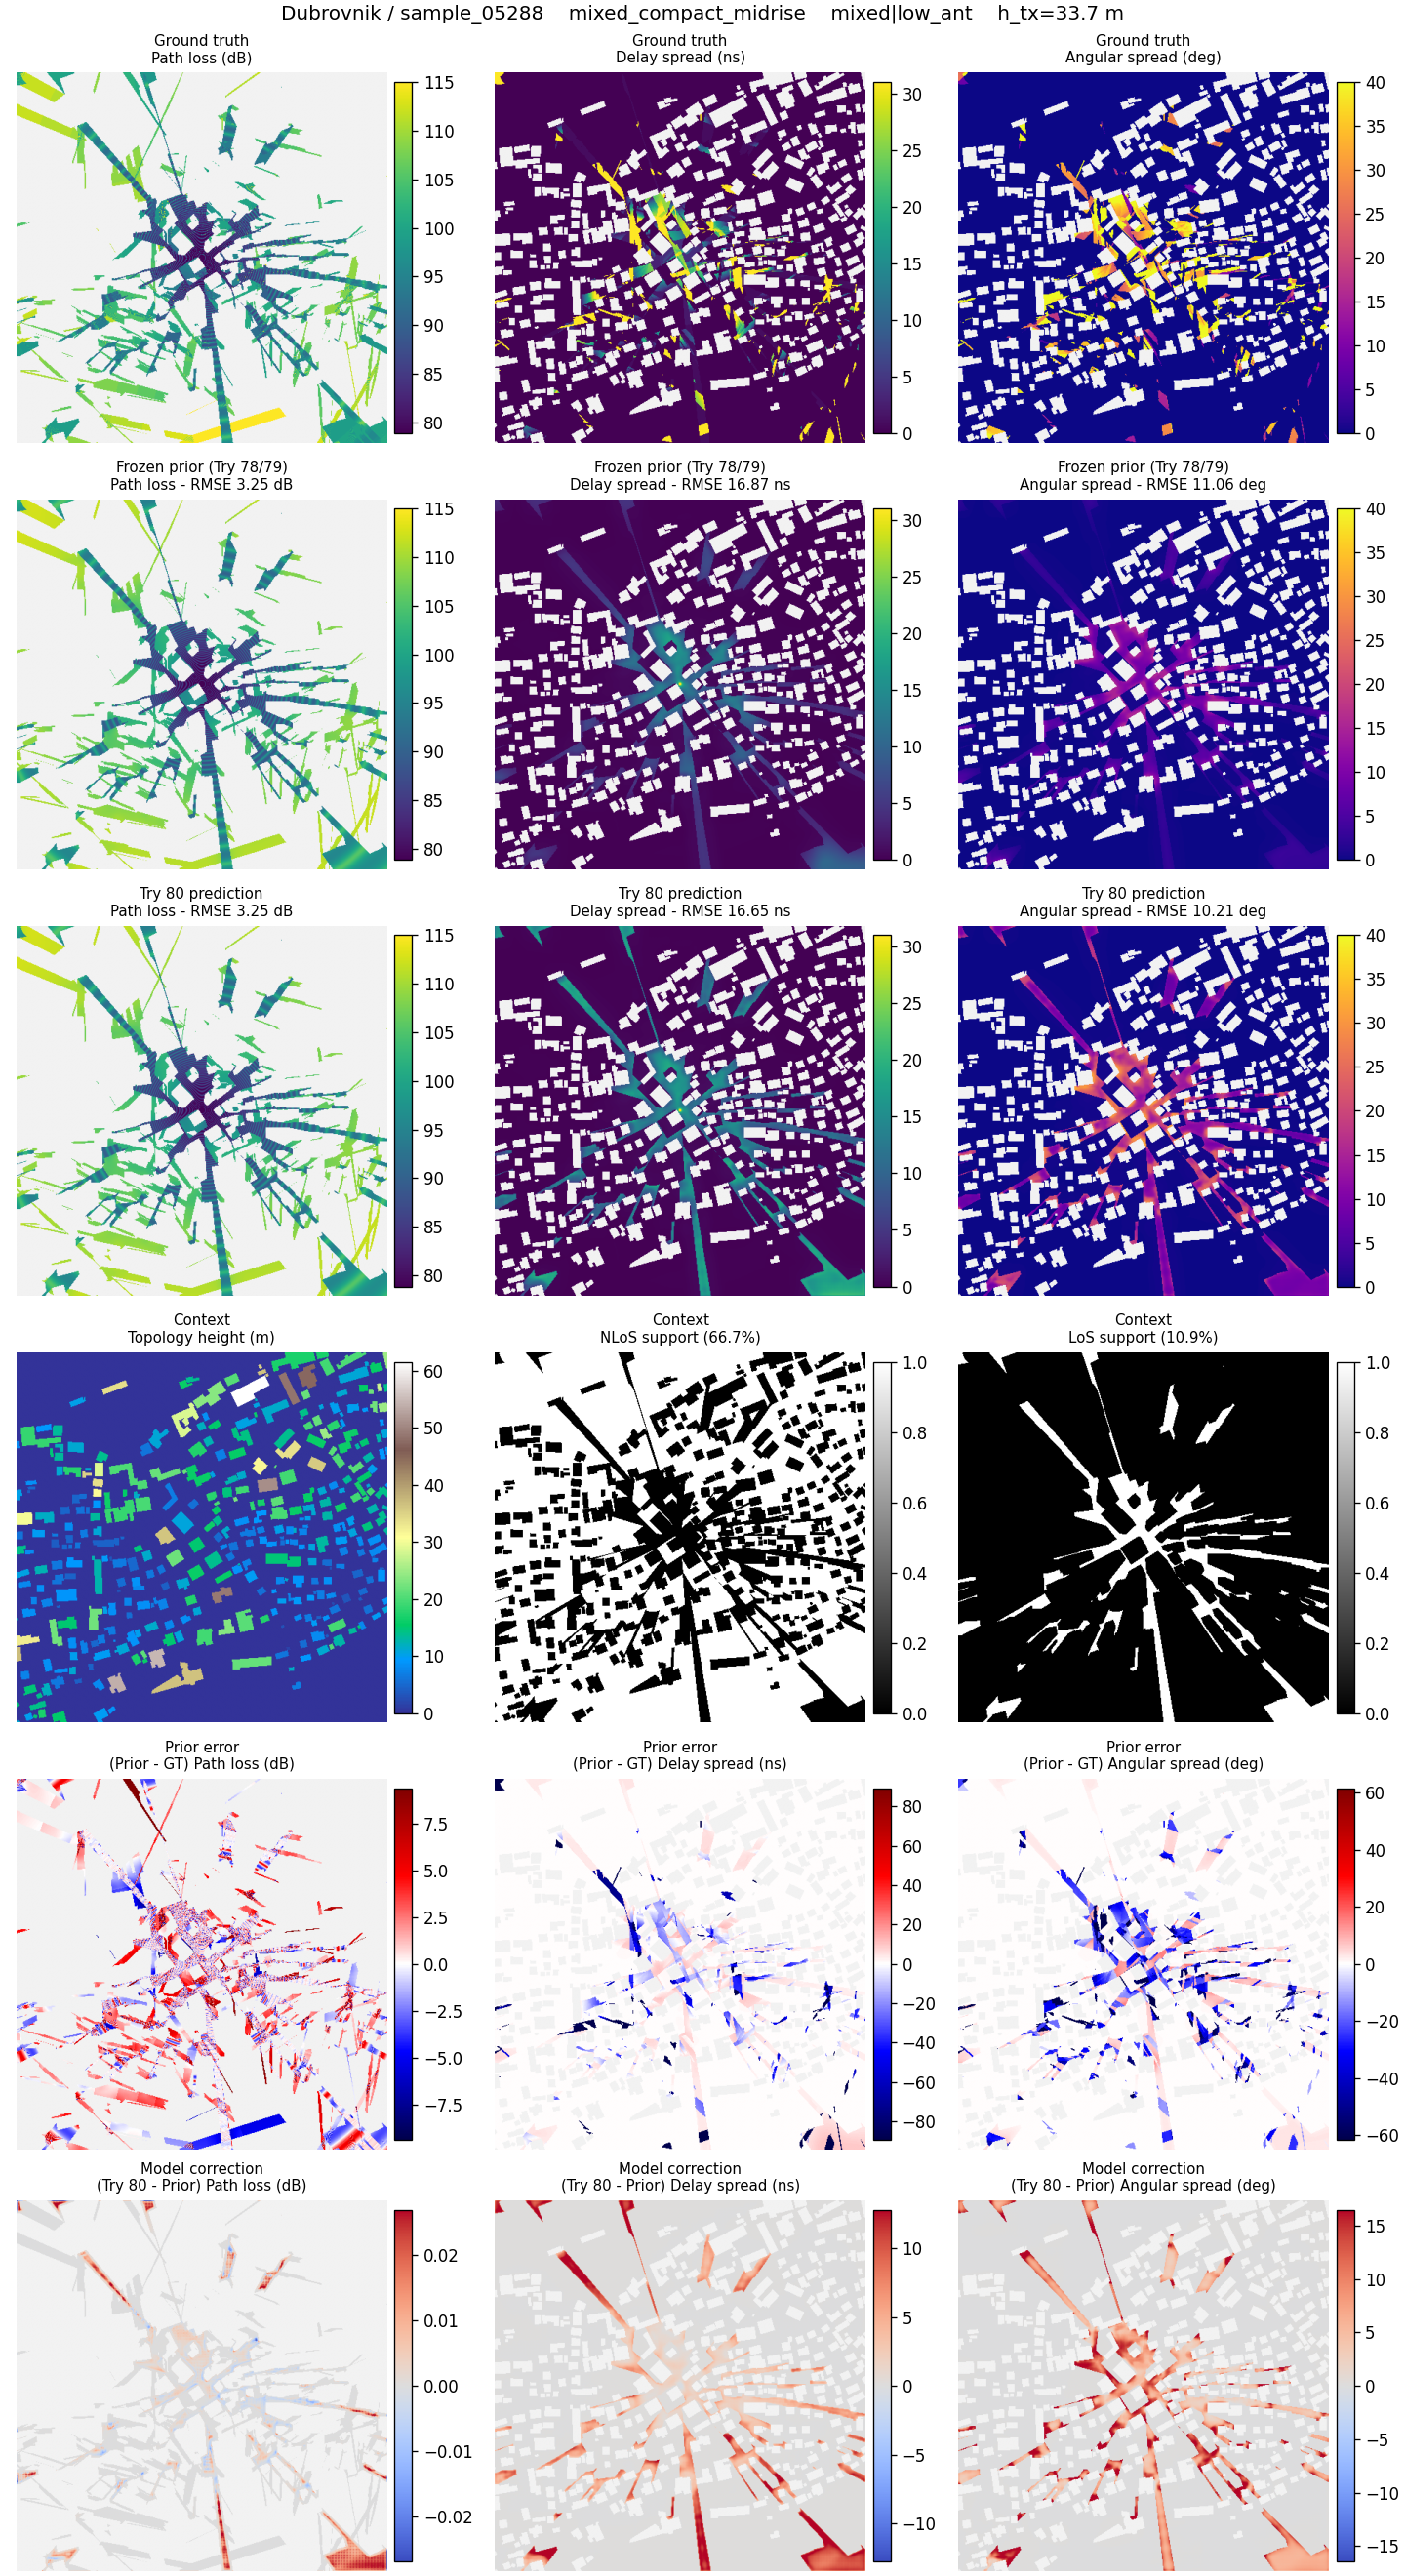
\includegraphics[width=\textwidth,height=0.88\textheight,keepaspectratio]{img/thesis_figures/try80_appendix_panels/try80_panel_mixed_low_ant_Dubrovnik_sample_05288_6x3.png}
\caption{Try 80 \(6\times3\) inspection panel for a mixed, low-antenna
validation sample in Dubrovnik.}
\label{fig:appendix_try80_mixed_low}
\end{figure}

\clearpage
\begin{figure}[p]
\centering
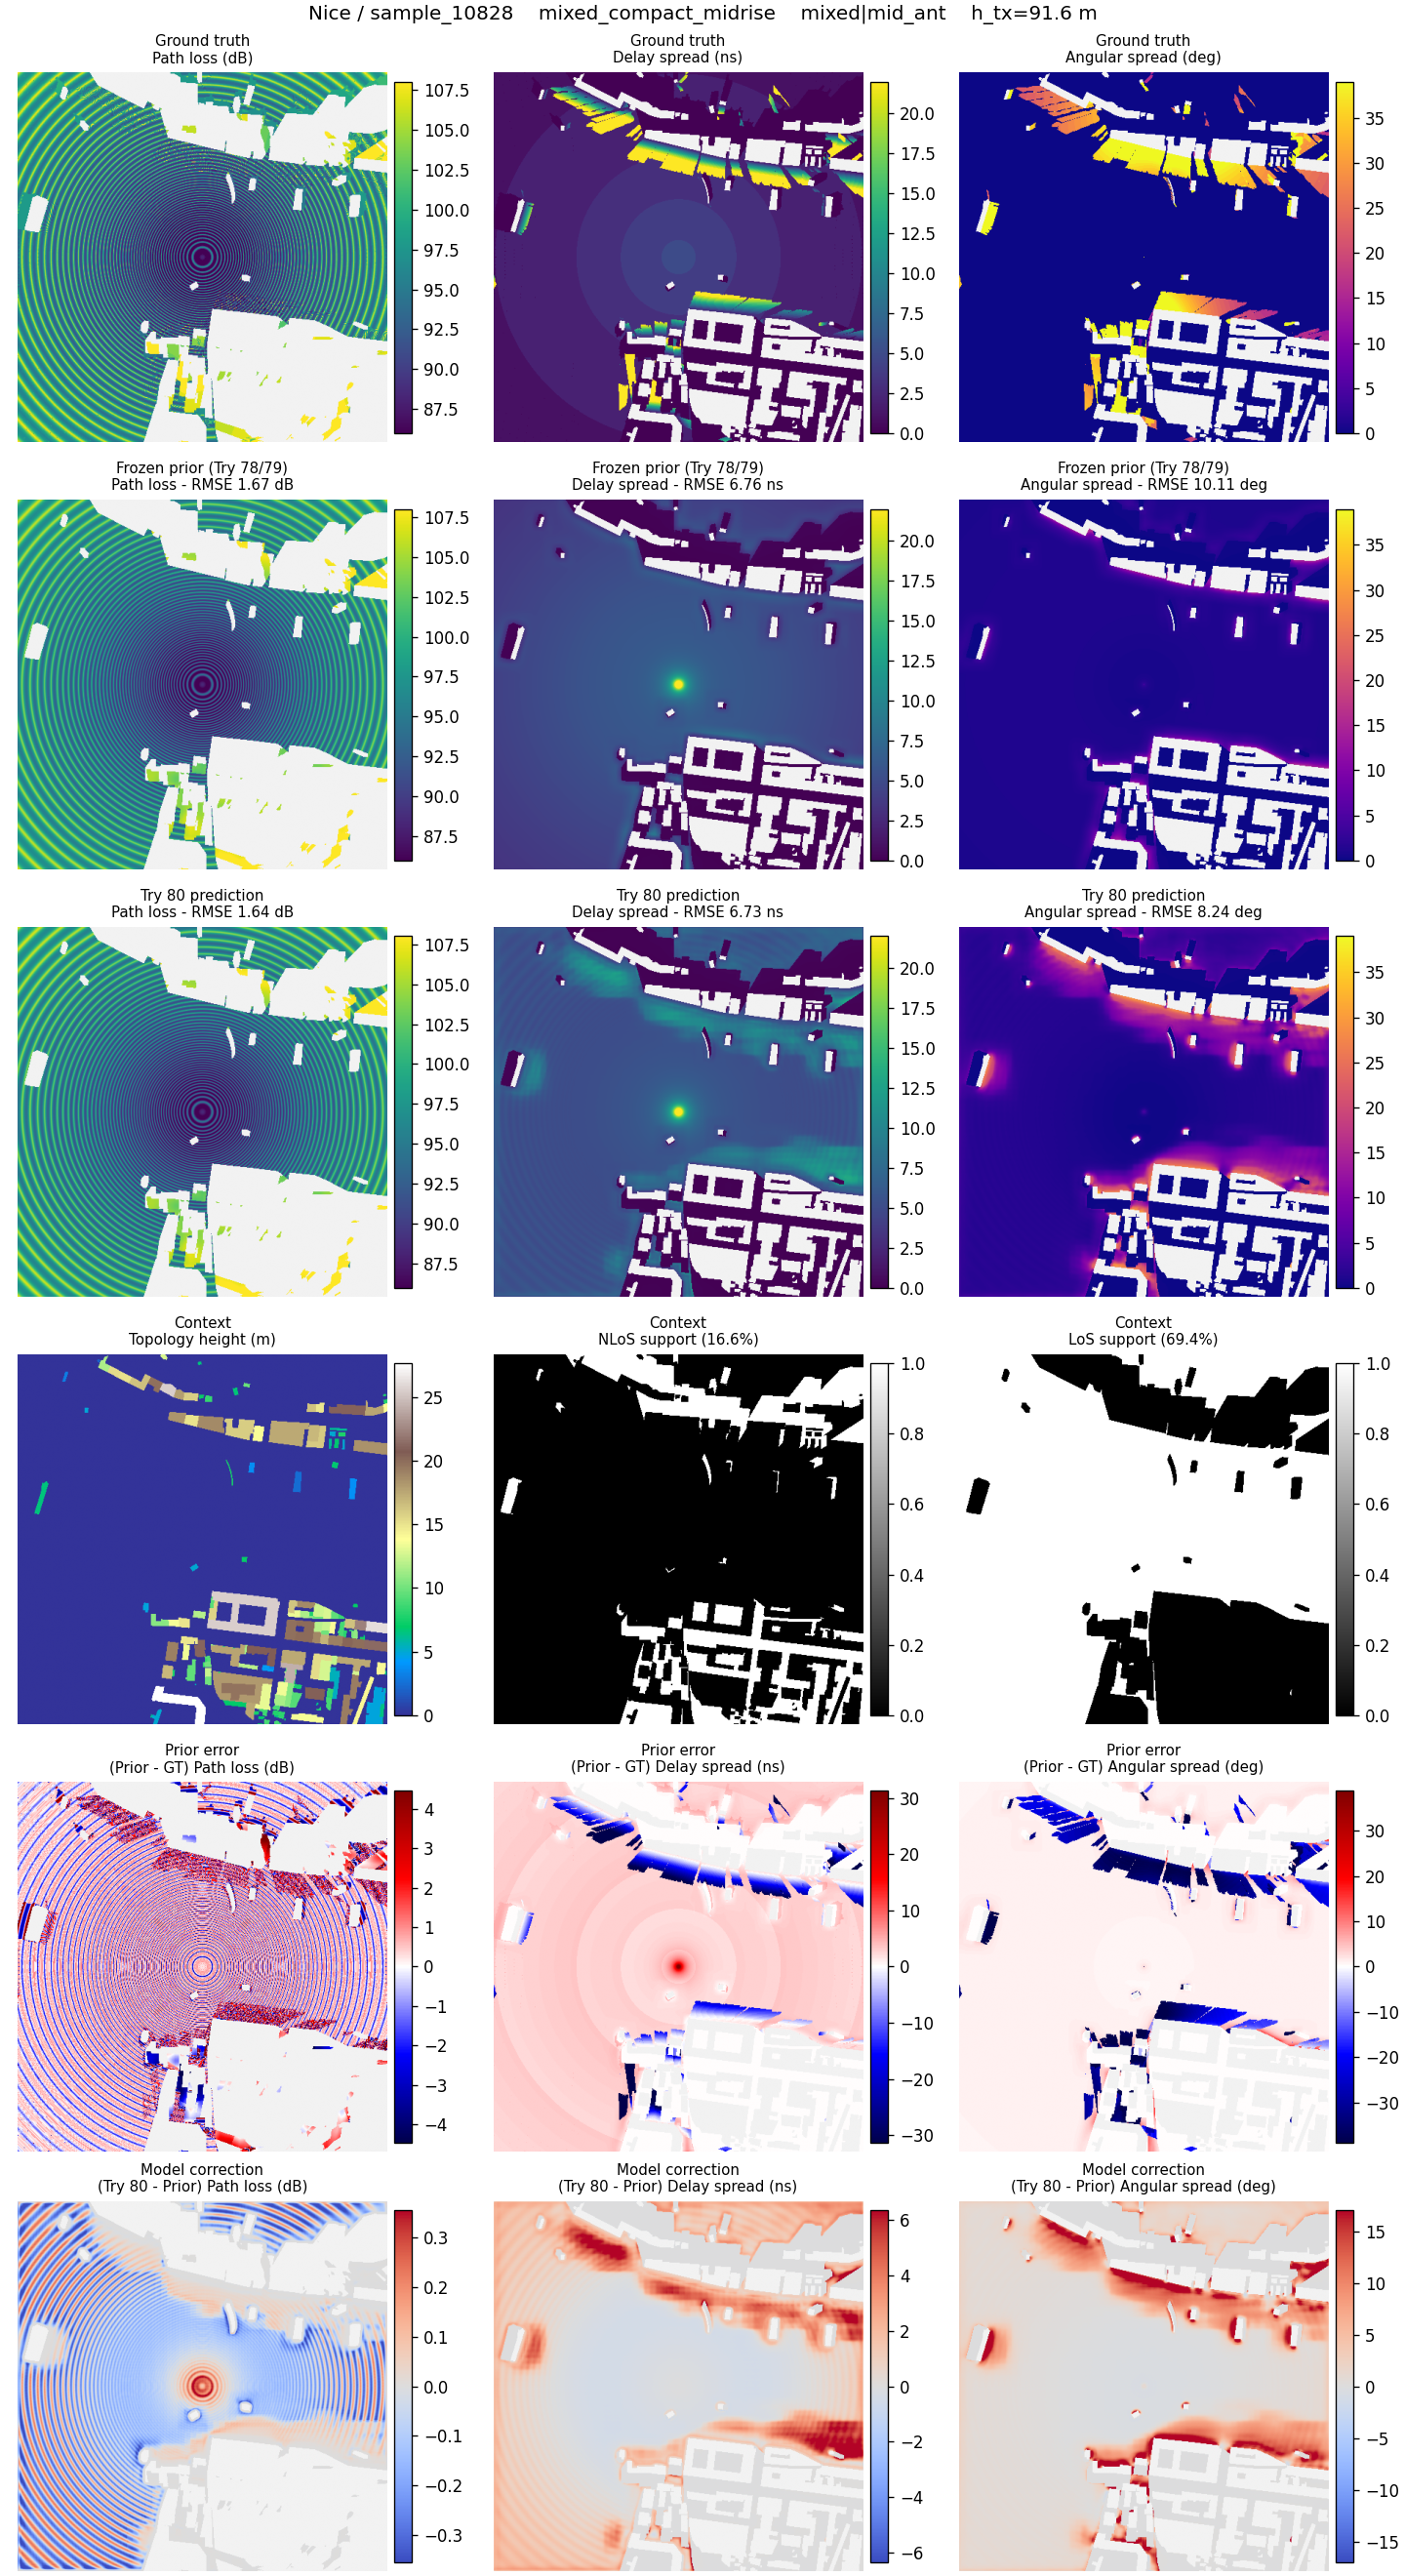
\includegraphics[width=\textwidth,height=0.88\textheight,keepaspectratio]{img/thesis_figures/try80_appendix_panels/try80_panel_mixed_mid_ant_Nice_sample_10828_6x3.png}
\caption{Try 80 \(6\times3\) inspection panel for a mixed, mid-antenna
validation sample in Nice.}
\label{fig:appendix_try80_mixed_mid}
\end{figure}

\clearpage
\begin{figure}[p]
\centering
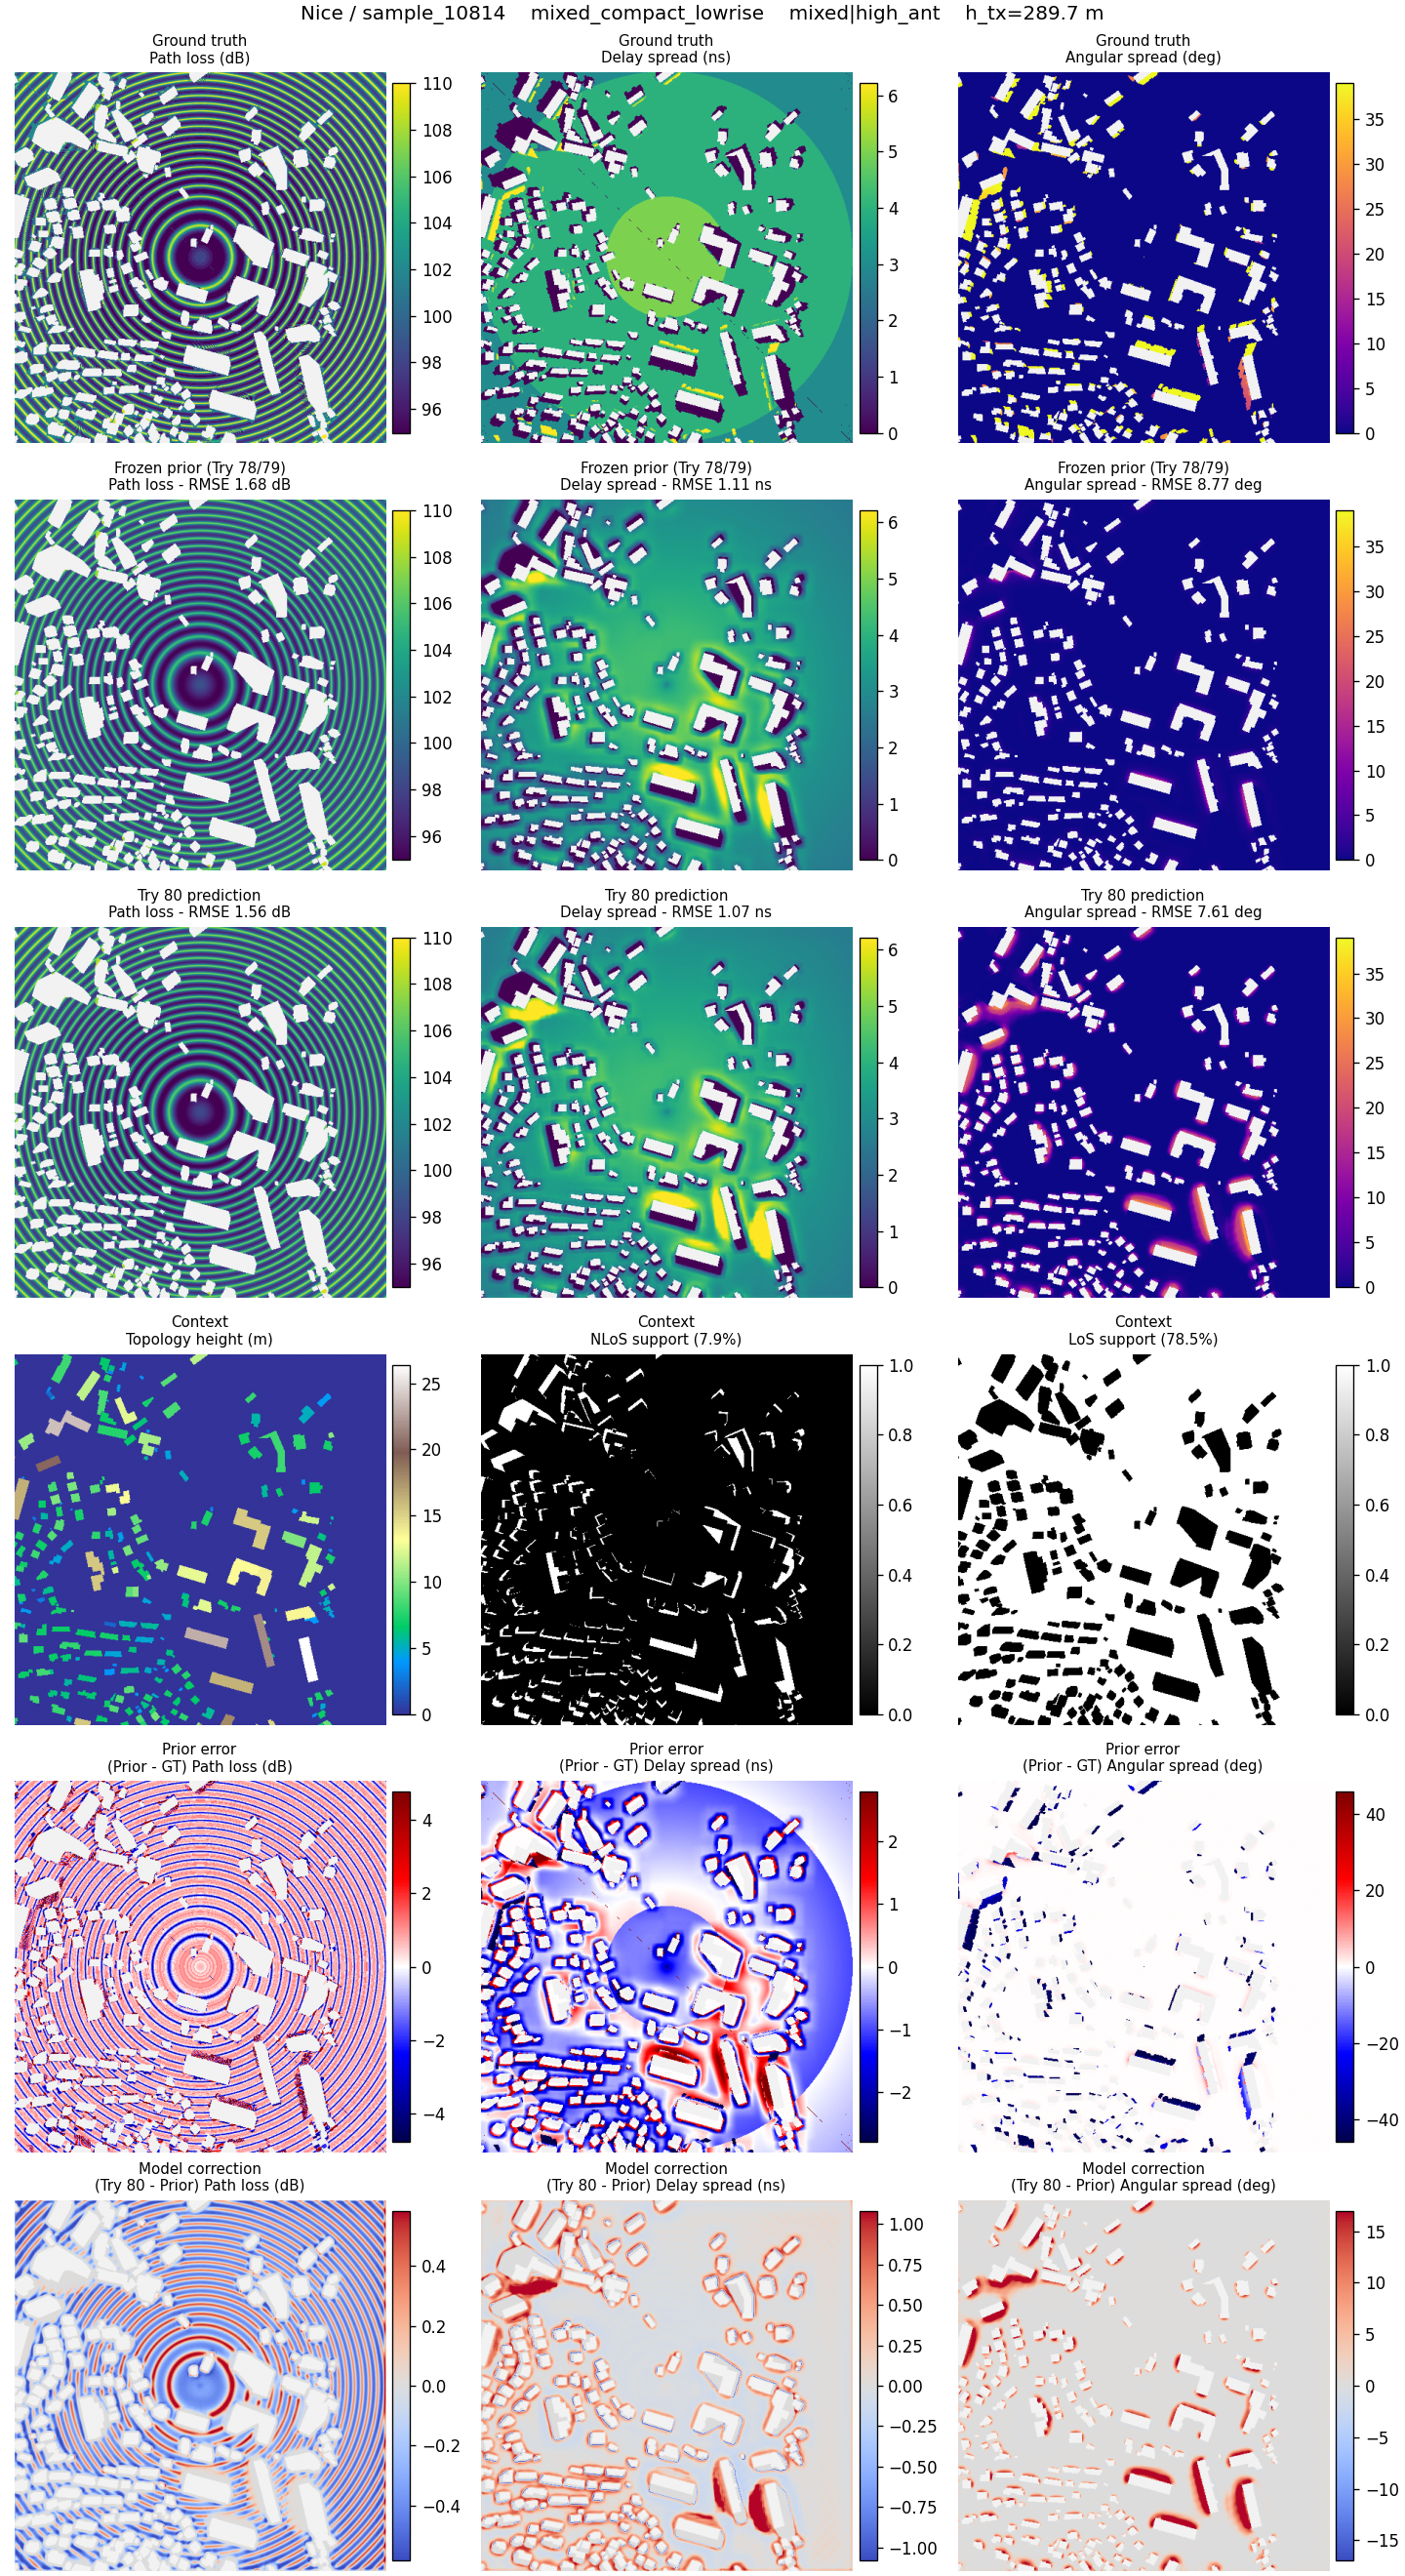
\includegraphics[width=\textwidth,height=0.88\textheight,keepaspectratio]{img/thesis_figures/try80_appendix_panels/try80_panel_mixed_high_ant_Nice_sample_10814_6x3.png}
\caption{Try 80 \(6\times3\) inspection panel for a mixed, high-antenna
validation sample in Nice.}
\label{fig:appendix_try80_mixed_high}
\end{figure}

\clearpage
\begin{figure}[p]
\centering
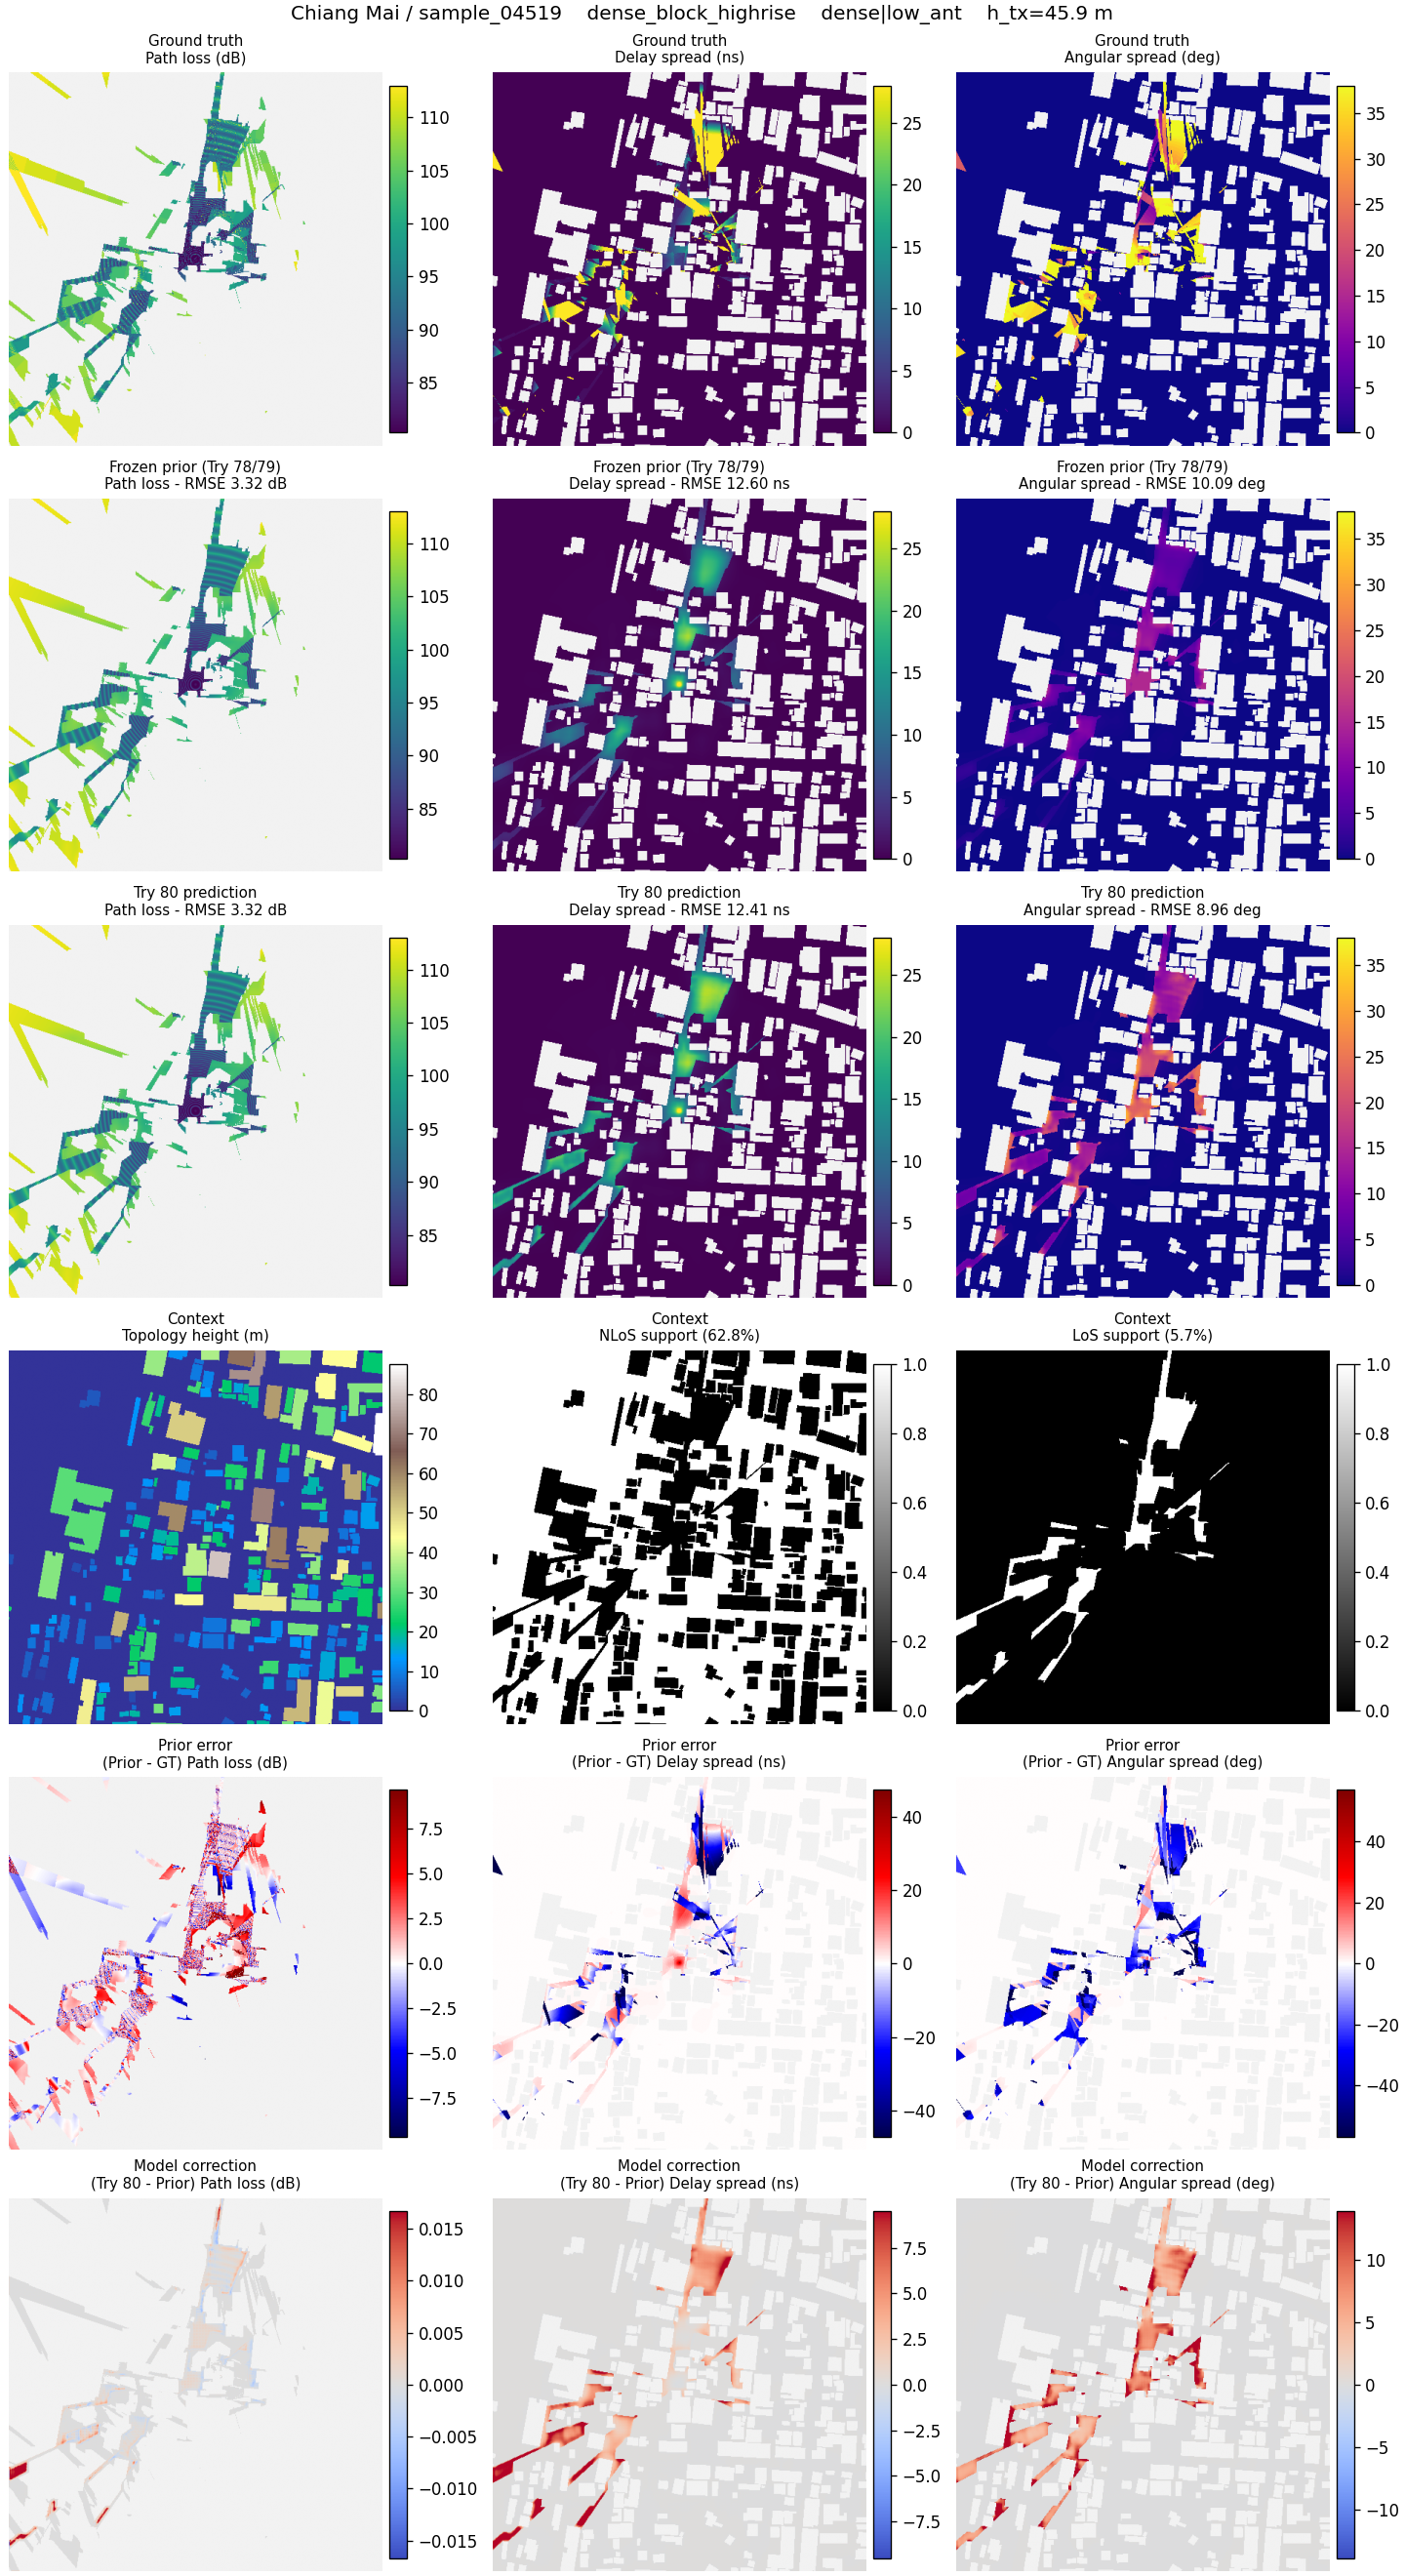
\includegraphics[width=\textwidth,height=0.88\textheight,keepaspectratio]{img/thesis_figures/try80_appendix_panels/try80_panel_dense_low_ant_Chiang_Mai_sample_04519_6x3.png}
\caption{Try 80 \(6\times3\) inspection panel for a dense, low-antenna
validation sample in Chiang Mai.}
\label{fig:appendix_try80_dense_low}
\end{figure}

\clearpage
\begin{figure}[p]
\centering
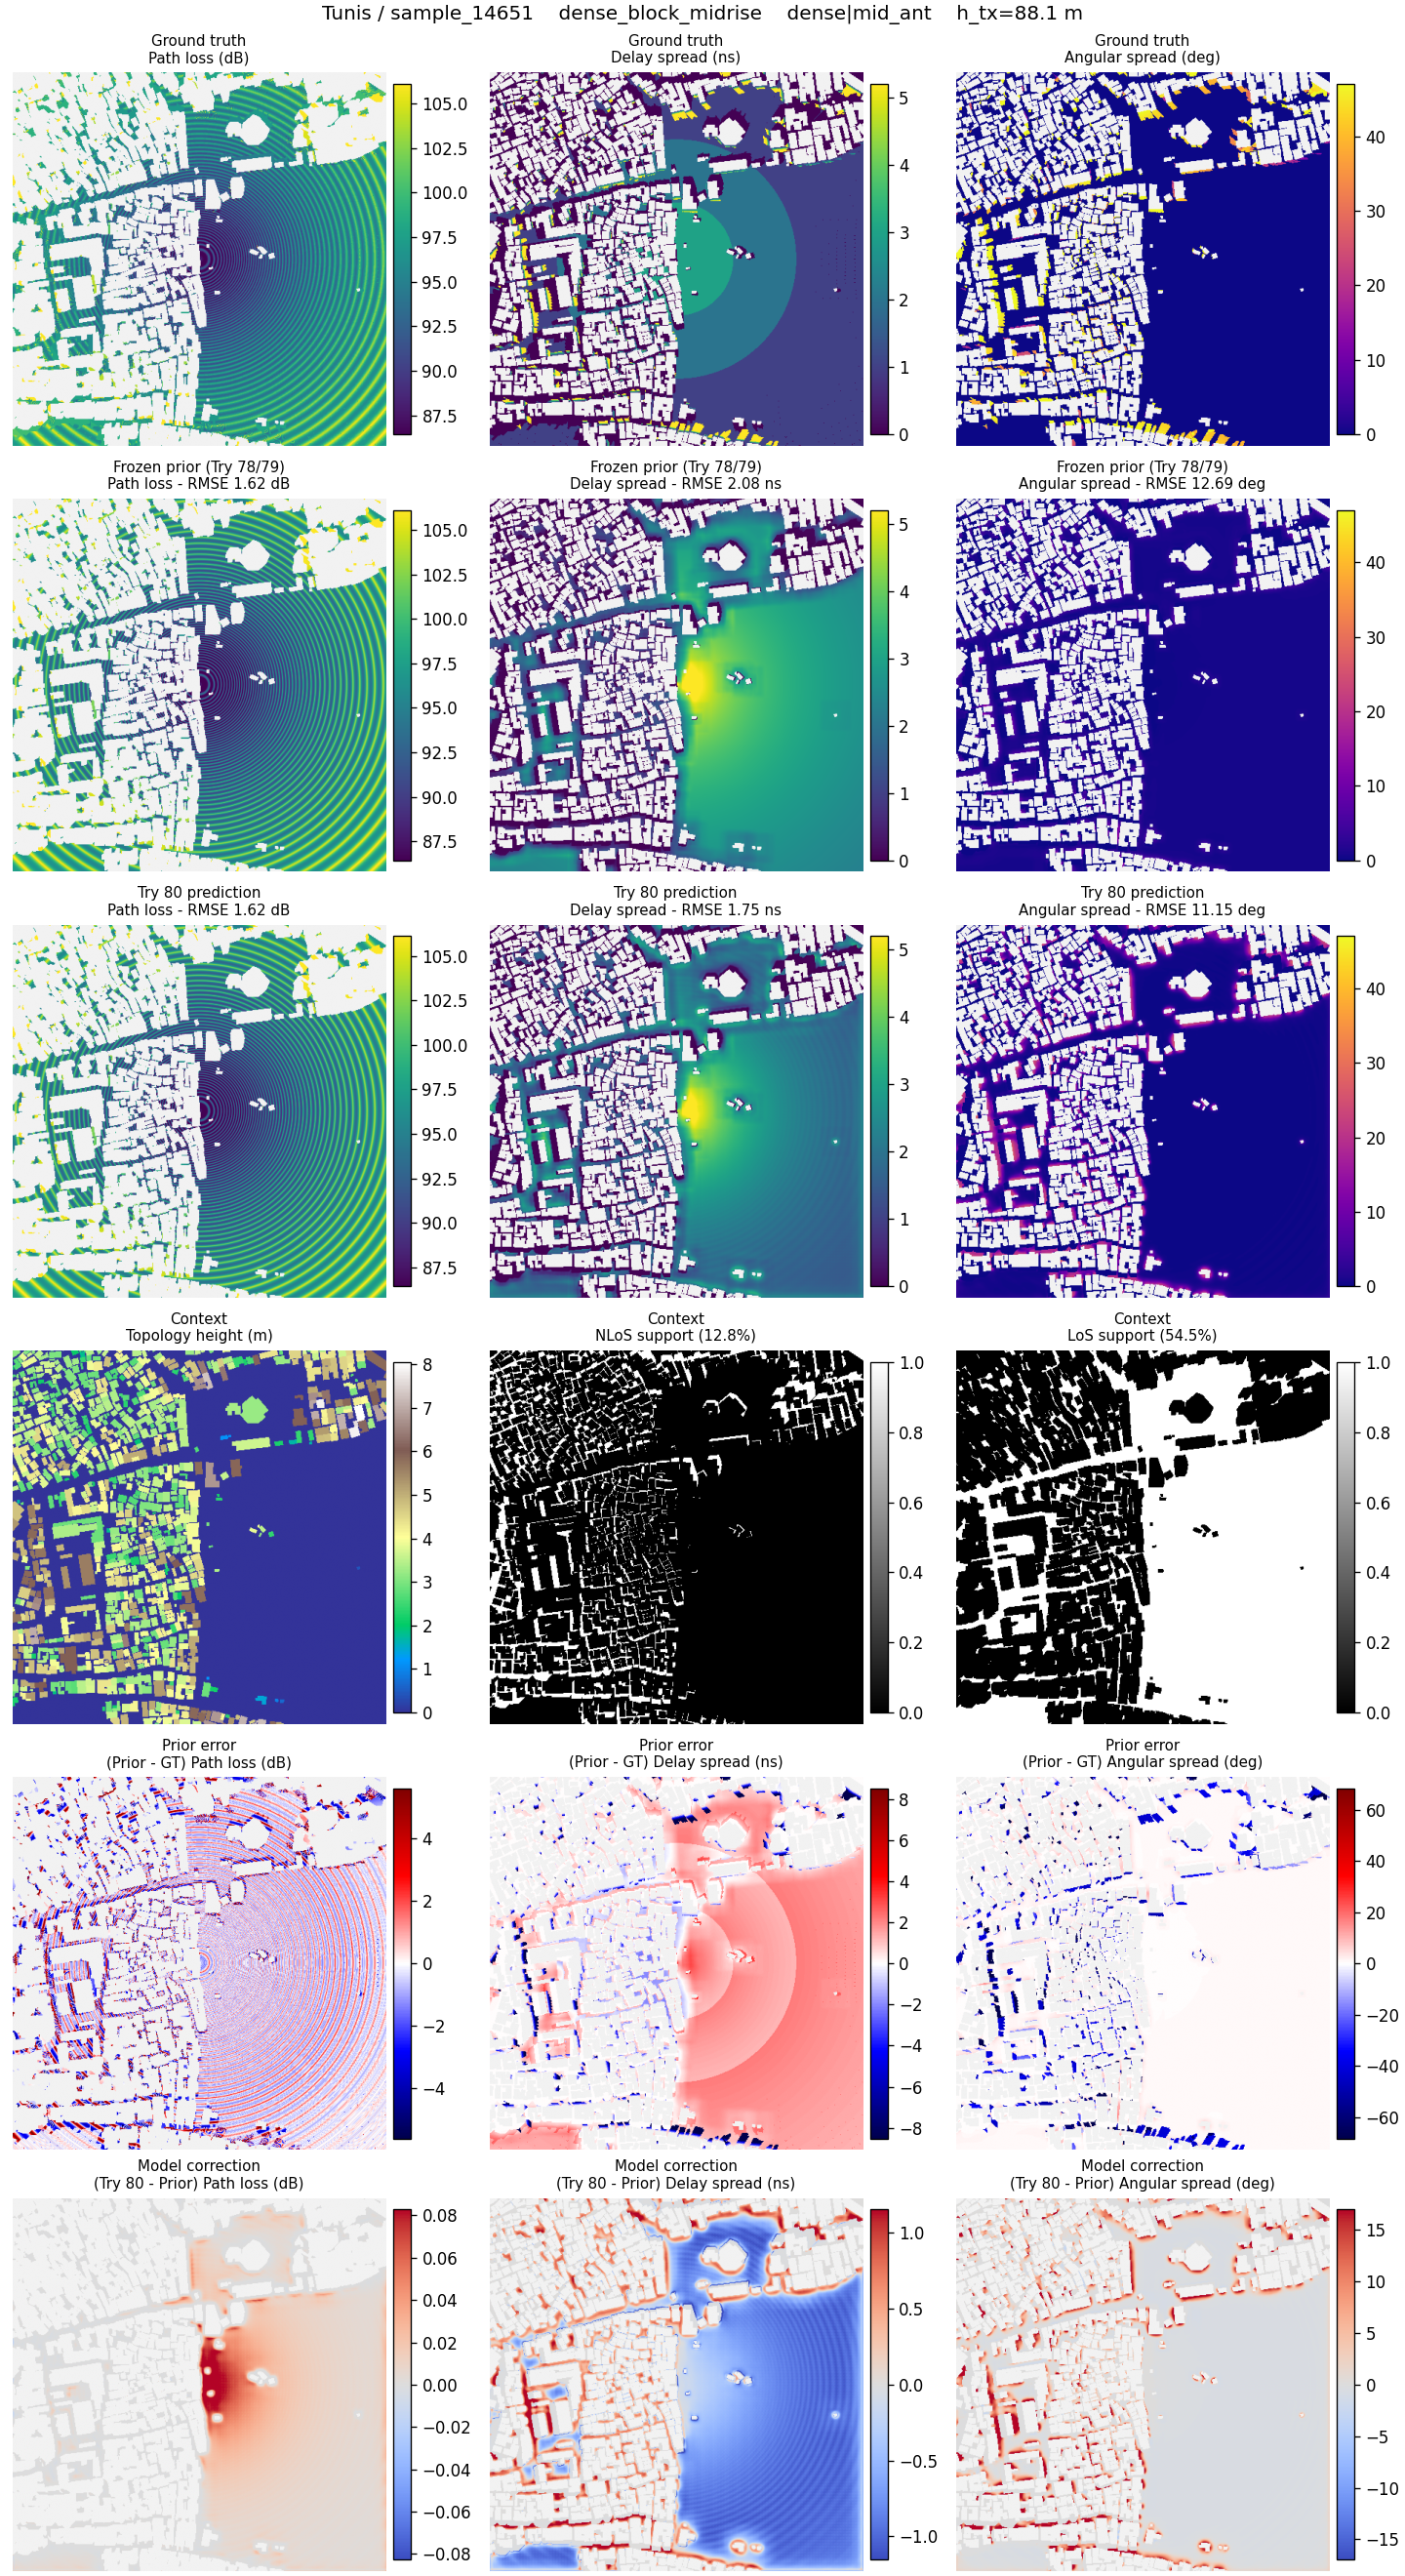
\includegraphics[width=\textwidth,height=0.88\textheight,keepaspectratio]{img/thesis_figures/try80_appendix_panels/try80_panel_dense_mid_ant_Tunis_sample_14651_6x3.png}
\caption{Try 80 \(6\times3\) inspection panel for a dense, mid-antenna
validation sample in Tunis.}
\label{fig:appendix_try80_dense_mid}
\end{figure}

\clearpage
\begin{figure}[p]
\centering
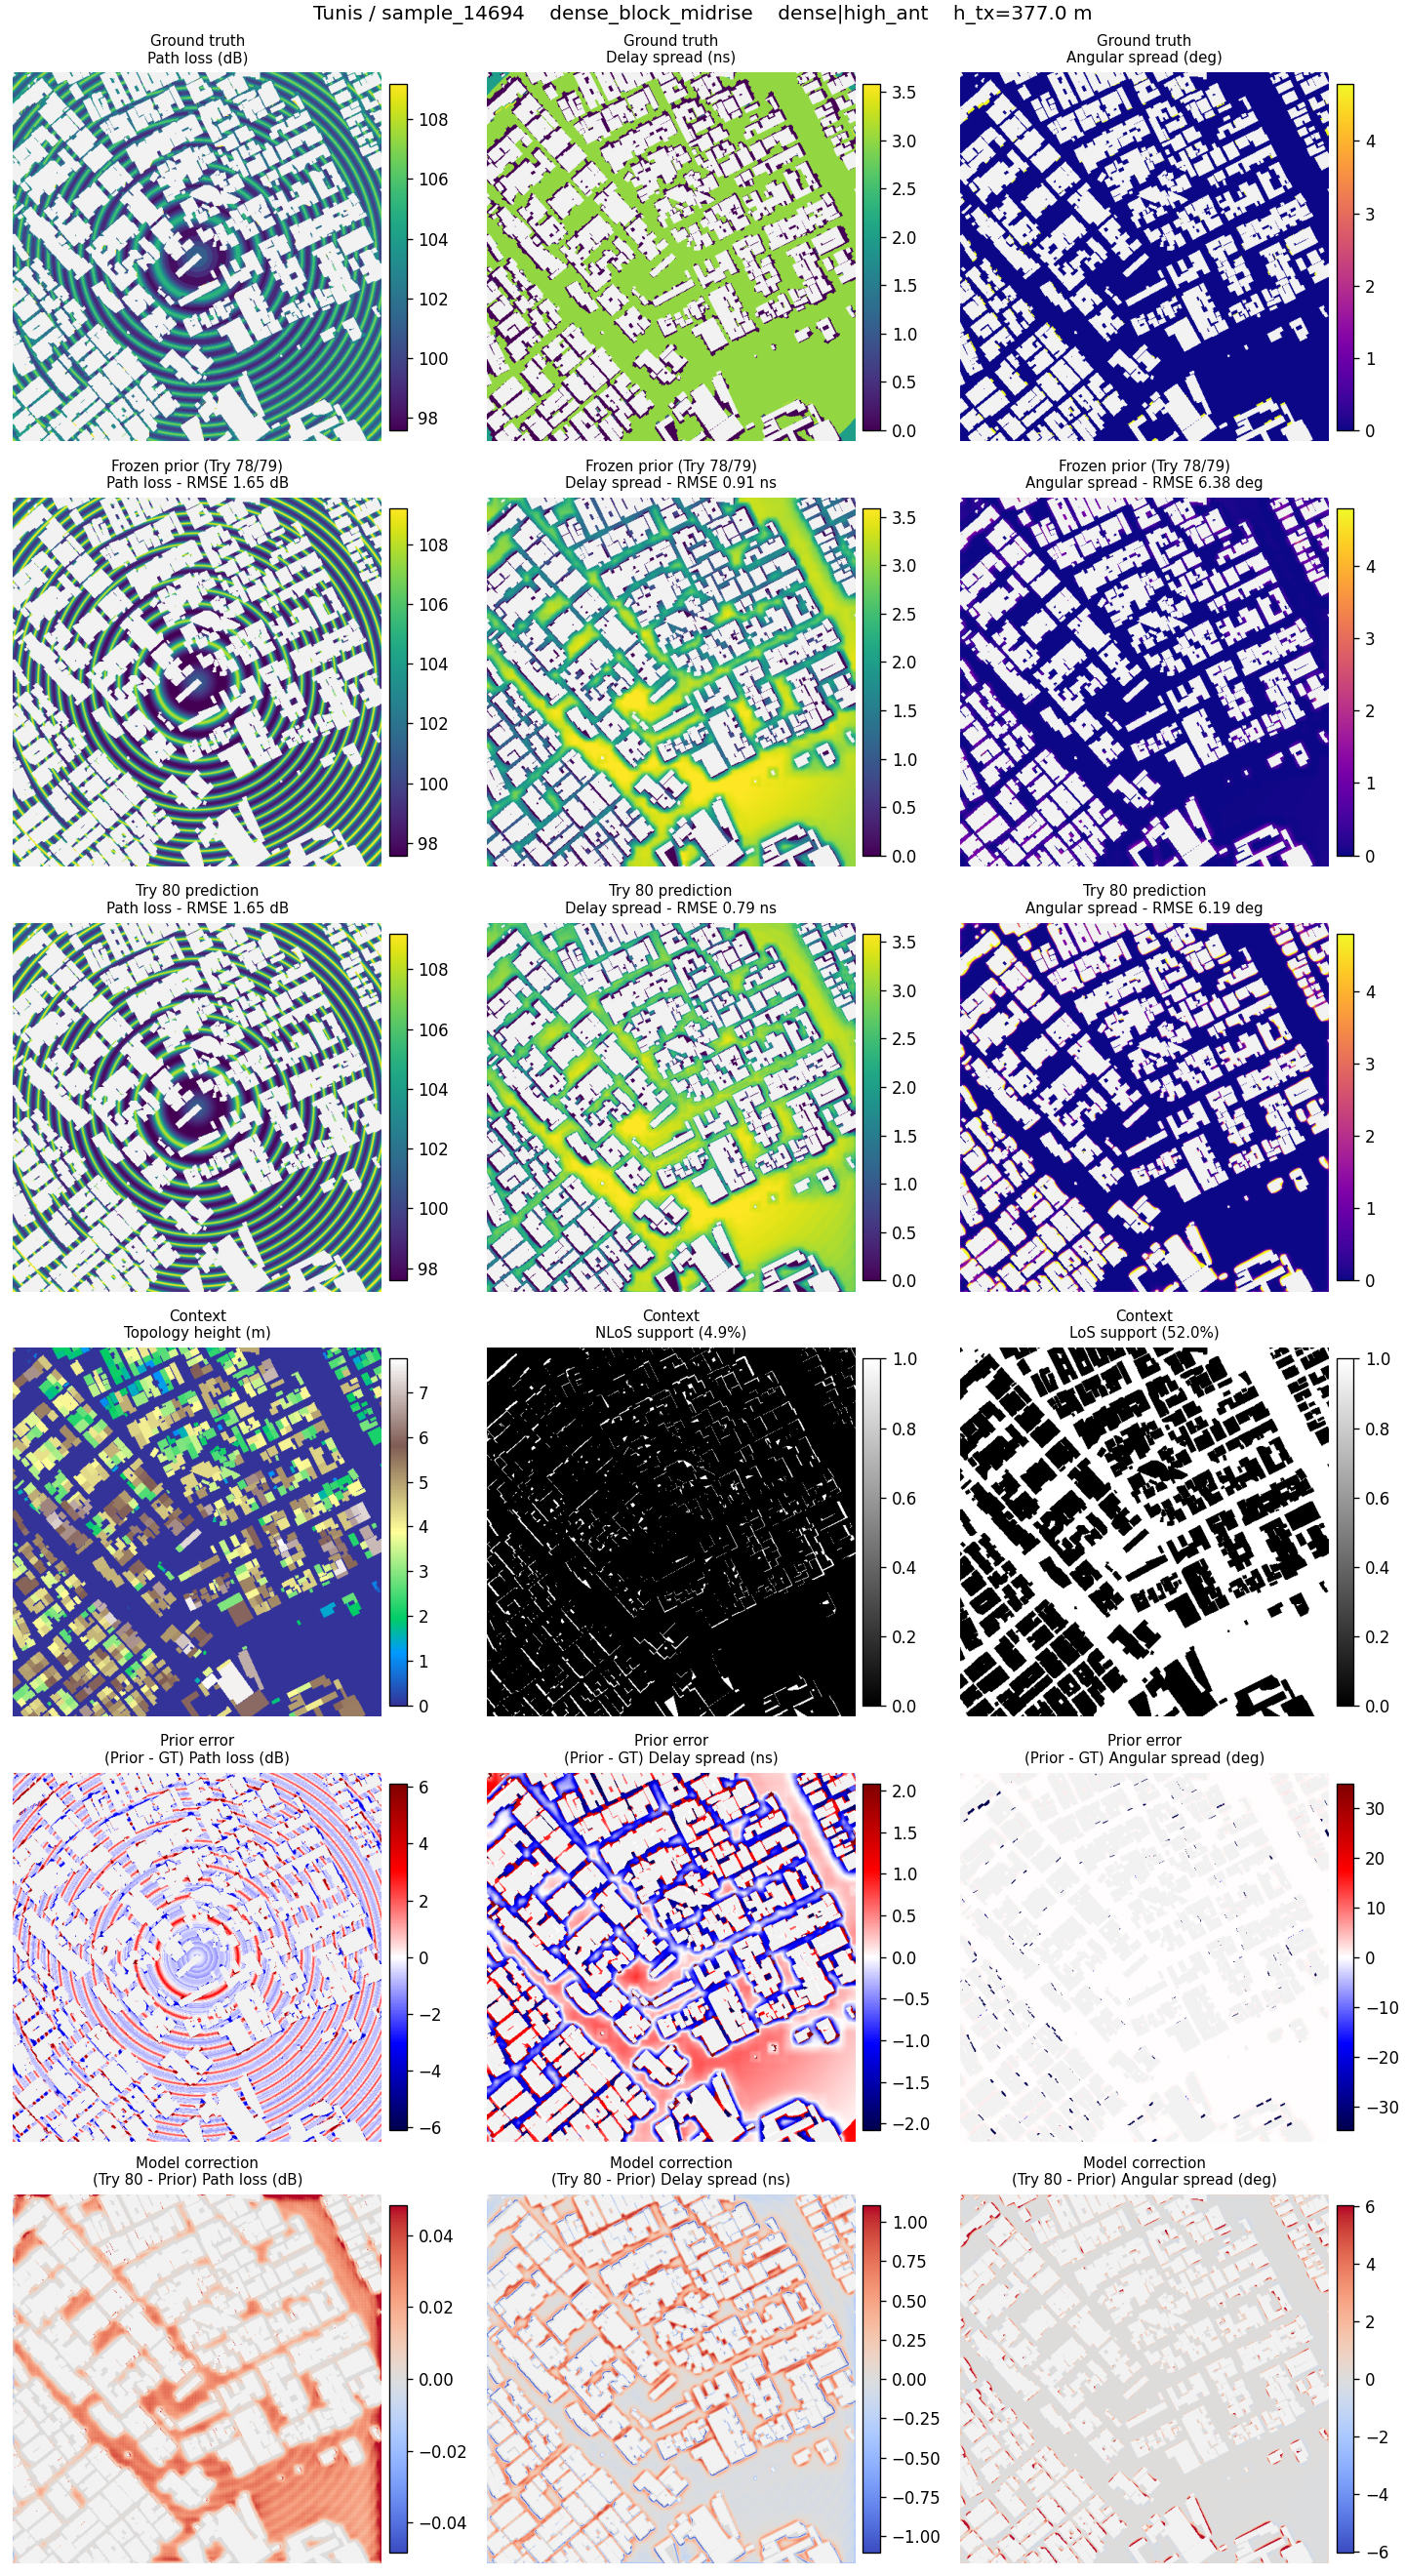
\includegraphics[width=\textwidth,height=0.88\textheight,keepaspectratio]{img/thesis_figures/try80_appendix_panels/try80_panel_dense_high_ant_Tunis_sample_14694_6x3.png}
\caption{Try 80 \(6\times3\) inspection panel for a dense, high-antenna
validation sample in Tunis.}
\label{fig:appendix_try80_dense_high}
\end{figure}

\clearpage
\chapter{Implementation Snippets}

The full implementation remains in the repository; the snippets below include
only the parts most relevant for reproducing the prior-anchored Try 80 design.
They are included here so the appendix contains the bridge between the formulas
in Chapter~3 and the code that produced the reported figures.

\section{Frozen prior assembly}

The Try 80 prior computer combines the calibrated Try 78 path-loss prior with
the calibrated Try 79 spread priors. The path-loss branch keeps separate LoS
and NLoS estimates, then blends them with the visibility mask:

{\scriptsize
\begin{verbatim}
ct6 = classify_topology(topology)
ct3 = macro_topology_class(ct6)
ant = ant_bin(h_tx)

los_prior = _predict_two_ray_map(h_tx, self._path_los_cal)
nlos_prior = _compute_try78_nlos_map(topology, los_mask, h_tx,
                                     self._path_nlos_cal)
path_prior = np.where(los_mask > 0.5, los_prior, nlos_prior)

delay_prior = _compute_try79_metric_prior("delay_spread", ct6, ant,
                                          los_mask, shared, self._spread_cal)
angular_prior = _compute_try79_metric_prior("angular_spread", ct6, ant,
                                            los_mask, shared, self._spread_cal)
\end{verbatim}
}

\section{Try 80 input tensor}

Each sample is passed to the model as nine aligned channels. The first four
channels describe geometry and support masks; the last five channels are the
frozen priors, normalized to stable numeric ranges:

{\scriptsize
\begin{verbatim}
channels = np.stack([
    topology_input,
    los,
    nlos,
    ground_f,
    path_prior / 180.0,
    path_prior_los / 180.0,
    path_prior_nlos / 180.0,
    np.log1p(np.clip(delay_prior, 0.0, None)) / LOG1P_DELAY_NORM,
    np.log1p(np.clip(angular_prior, 0.0, None)) / LOG1P_ANGULAR_NORM,
], axis=0)
\end{verbatim}
}

\section{Bounded residual decoder}

The model does not predict an unconstrained map. It predicts bounded residuals
around the prior, with separate LoS and NLoS residual limits and a learned
local gate \(\alpha\). For the spread targets, residuals are capped in native
units and then mapped back to the log domain:

{\scriptsize
\begin{verbatim}
residual_max_native = self.residual_max[task].to(device)
residual_max_native = residual_max_native.view(1, 2, 1, 1, 1)

global_delta_native = torch.tanh(global_raw["delta_mu_raw"])
global_delta_native = global_delta_native * residual_max_native

local_delta_native = torch.tanh(local_raw["local_delta_raw"])
local_delta_native = local_delta_native * residual_max_native
alpha = torch.sigmoid(local_raw["alpha_logits"] + self.cfg.alpha_bias)

delta_total_native = torch.clamp(global_delta_native + local_delta_native,
                                 min=-residual_max_native,
                                 max=residual_max_native)

mu_native = (prior_native_region + alpha * delta_total_native).clamp_min(0.0)
mu = torch.log1p(mu_native)
pred_region = (p * mu).sum(dim=2)
pred = (pred_region * region_masks.squeeze(2)).sum(dim=1, keepdim=True)
\end{verbatim}
}

\chapter{CKM Generator Interface and Reproducibility Tool}
\label{app:ckm_generator}

This appendix documents the standalone CKM Generator delivered with the final
Try~80 pipeline. The tool was built to make the trained model usable outside
the training scripts: it accepts topology inputs, prepares them with the same
geometric conventions used in the thesis, computes or imports LoS/NLoS masks,
evaluates the frozen Try~78/79 priors, optionally runs the Try~80 neural model,
and exports both visual figures and numerical arrays.

The generator is intentionally available through two front ends. The Streamlit
application is designed for inspection, rapid manual testing, and demonstrations
with uploaded files. The command-line interface uses the same backend and is
intended for reproducible scripted runs, validation, and larger batches.

\section{Interface overview}

Figure~\ref{fig:ckm_generator_controls} shows the main controls exposed by the
Streamlit interface. The left sidebar controls the input source, antenna height,
runtime device, mask policy, model execution, export format, image scaling,
pixel spacing, HDF5 filtering, and output folder.

\begin{figure}[H]
\centering

\includegraphics[width=\textwidth,height=0.72\textheight,keepaspectratio]{img/thesis_figures/ckm_generator/ckm_generator_app_controls.png}
\caption{CKM Generator Streamlit interface. The sidebar exposes the same
settings that are available through the command-line interface.}
\label{fig:ckm_generator_controls}
\end{figure}

After generation, the application presents the fitted topology next to the
LoS and NLoS masks actually used by the priors and model. This is important
because the masks are not only visual outputs: they are part of the Try~80
input tensor and determine the receiver-valid support used by the priors.
Figure~\ref{fig:ckm_generator_masks} shows this inspection view.

\begin{figure}[H]
\centering
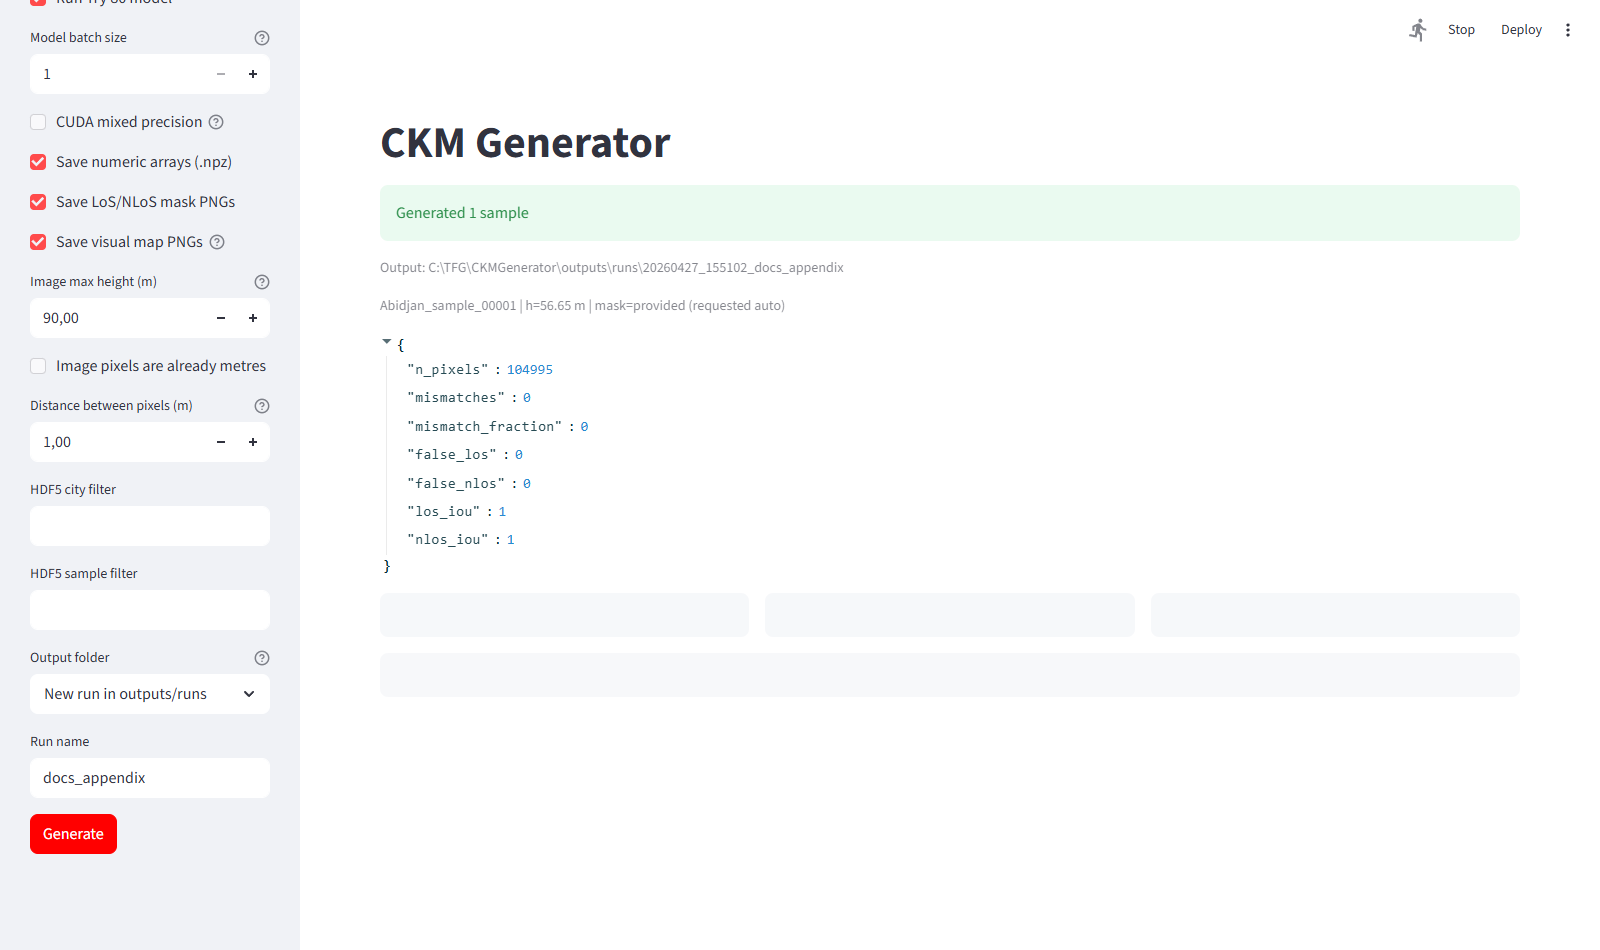
\includegraphics[width=\textwidth,height=0.72\textheight,keepaspectratio]{img/thesis_figures/ckm_generator/ckm_generator_app_result_top.png}
\caption{Generated topology and masks for an HDF5 sample. The view reports
the resolved mask source and displays topology, LoS mask, and NLoS mask
side by side.}
\label{fig:ckm_generator_masks}
\end{figure}

When the Try~80 model is enabled, the generator produces the three target
maps in their native units. Figure~\ref{fig:ckm_generator_prediction} shows
the joint prediction panel saved by the tool.

\begin{figure}[H]
\centering
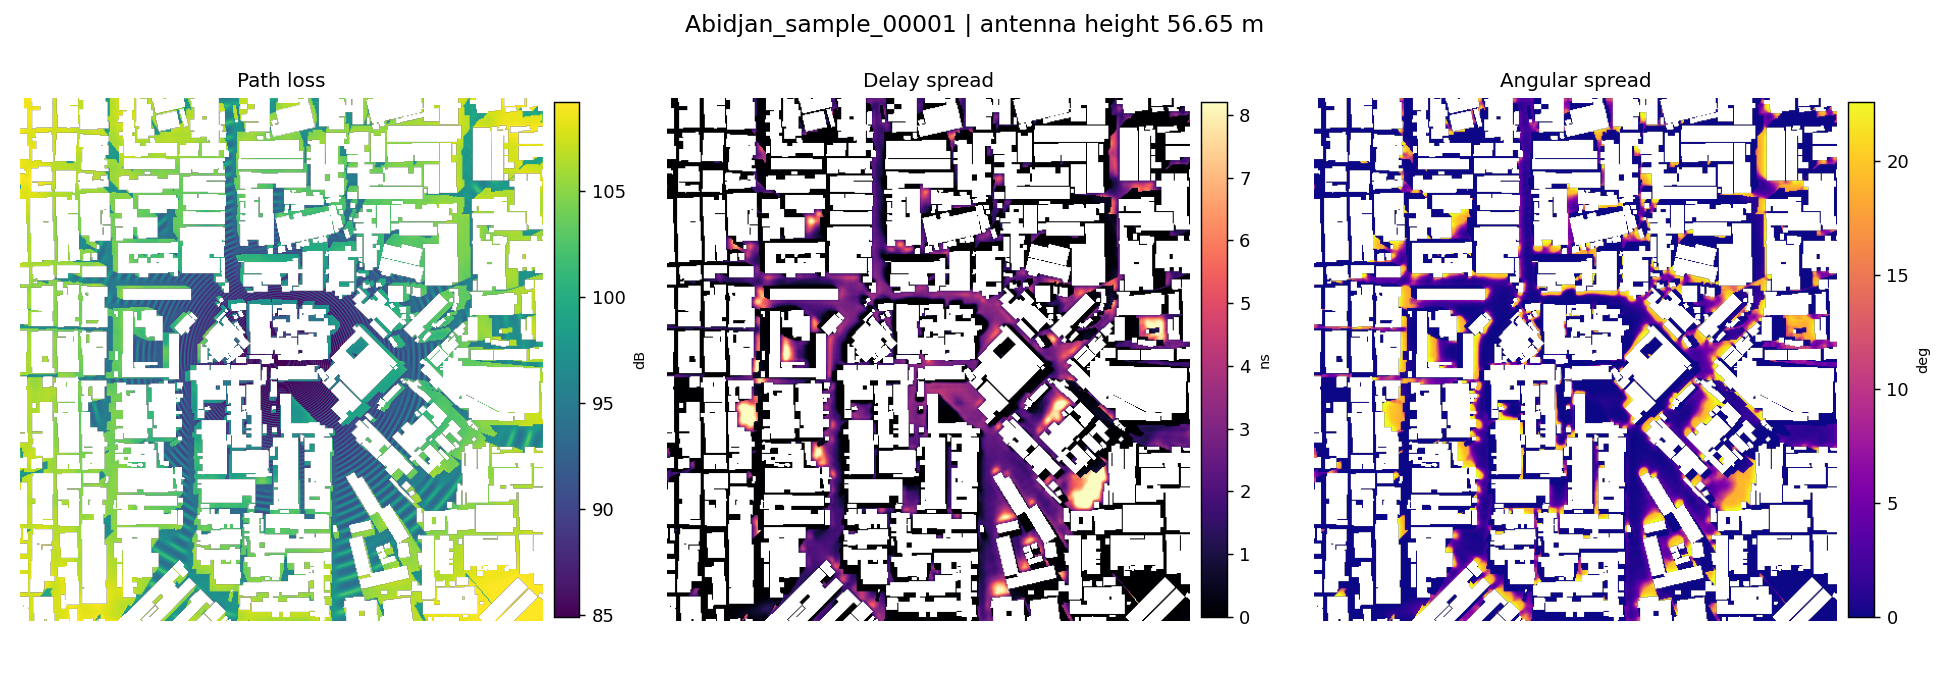
\includegraphics[width=\textwidth,height=0.72\textheight,keepaspectratio]{img/thesis_figures/ckm_generator/ckm_generator_prediction_joint.png}
\caption{Joint prediction figure exported by the CKM Generator, with path
loss in dB, delay spread in ns, and angular spread in degrees.}
\label{fig:ckm_generator_prediction}
\end{figure}

\section{How the tool is run}

The dependencies are installed in the Python environment that will run the
tool:

{\scriptsize
\begin{verbatim}
cd C:\TFG\CKMGenerator
C:\Python310\python.exe -m pip install -r C:\TFG\CKMGenerator\requirements.txt
\end{verbatim}
}

The runtime check is executed before inference:

{\scriptsize
\begin{verbatim}
C:\Python310\python.exe C:\TFG\CKMGenerator\ckm_doctor.py
\end{verbatim}
}

The doctor command checks PyTorch, CUDA, DirectML, the checkpoint, available
memory, and whether the selected runtime can execute the Try~80 model. In
\texttt{auto} mode, the runtime priority is CUDA, then DirectML, then CPU.

The Streamlit application is started with:

{\scriptsize
\begin{verbatim}
C:\Python310\python.exe -m streamlit run C:\TFG\CKMGenerator\ckm_app.py
\end{verbatim}
}

The equivalent terminal command for an HDF5 sample is:

{\scriptsize
\begin{verbatim}
C:\Python310\python.exe C:\TFG\CKMGenerator\ckm_generate.py ^
  --input C:\TFG\CKMGenerator\inputs\samples\Abidjan_sample_00001.h5 ^
  --run-name abidjan_check ^
  --mixed-precision
\end{verbatim}
}

For an image-only topology, the transmitter height must be supplied explicitly
unless it is stored in a structured input file:

{\scriptsize
\begin{verbatim}
C:\Python310\python.exe C:\TFG\CKMGenerator\ckm_generate.py ^
  --input C:\path\topology_map.png ^
  --height 56.65 ^
  --topology-max-m 120 ^
  --meters-per-pixel 1.0 ^
  --mask-source auto ^
  --mixed-precision
\end{verbatim}
}

\section{Accepted inputs}

The generator accepts three families of input files:

\begin{itemize}
\setlength\itemsep{0.15em}
  \item Raster topology images: \texttt{.png}, \texttt{.jpg},
        \texttt{.jpeg}, \texttt{.tif}, \texttt{.tiff}, and \texttt{.bmp}.
  \item Numeric arrays: \texttt{.npy}, \texttt{.npz}, \texttt{.csv},
        \texttt{.txt}, and \texttt{.json}.
  \item HDF5 files: \texttt{.h5}, \texttt{.hdf5}, and \texttt{.hdf}.
\end{itemize}

For HDF5 and NPZ inputs, topology arrays are detected using the keys
\texttt{topology\_map}, \texttt{topology}, \texttt{building\_height},
\texttt{building\_heights}, \texttt{height\_map}, or \texttt{terrain}.
The optional LoS and NLoS masks can be read from \texttt{los\_mask},
\texttt{LoS\_mask}, \texttt{los}, \texttt{LoS}, \texttt{nlos\_mask},
\texttt{nLoS\_mask}, \texttt{NLoS\_mask}, \texttt{nlos}, or
\texttt{NLoS}. The optional antenna height can be read from
\texttt{uav\_height}, \texttt{antenna\_height},
\texttt{antenna\_height\_m}, \texttt{height}, \texttt{height\_m}, or
\texttt{h\_tx}.

For image or array topology files, sidecar masks are detected when they share
the same base name:

{\scriptsize
\begin{verbatim}
sample_topology.png
sample_los_mask.png
sample_nlos_mask.png
\end{verbatim}
}

The exported manual-input folder also uses a sibling \texttt{masks\_png}
directory, which is checked automatically. The valid transmitter-height range
is \SI{10}{m} to \SI{478}{m}. Receiver height is fixed at \SI{1.5}{m}, as in
the CKM calibration and in the Try~78/79/80 prior formulas.

\section{Configurable controls}

The Streamlit interface exposes the following operational controls:

\begin{itemize}
\setlength\itemsep{0.15em}
  \item \texttt{Local input path}: reads a file already present on disk.
  \item \texttt{Or upload topology / data / HDF5}: uploads one or more files.
  \item \texttt{Antenna height (m)}: used when height is not stored in the input.
  \item \texttt{Device}: selects \texttt{auto}, \texttt{cuda},
        \texttt{directml}, or \texttt{cpu}.
  \item \texttt{Mask used by priors/model}: selects \texttt{auto},
        \texttt{provided}, or \texttt{generated}.
  \item \texttt{Run Try 80 model}: disables neural inference when only masks
        and priors are needed.
  \item \texttt{Model batch size}: sends several prepared samples through the
        model in one forward pass when GPU memory allows it.
  \item \texttt{CUDA mixed precision}: enables CUDA autocast inference.
  \item \texttt{Save numeric arrays (.npz)}: exports all numeric arrays.
  \item \texttt{Save LoS/NLoS mask PNGs}: exports binary mask images.
  \item \texttt{Save visual map PNGs}: exports rendered prior and prediction
        figures with colour bars.
  \item \texttt{Image max height (m)}: scales image pixel values into metres.
  \item \texttt{Image pixels are already metres}: treats image pixel values as
        physical metre values and bypasses image normalisation.
  \item \texttt{Distance between pixels (m)}: physical input pixel spacing.
  \item \texttt{HDF5 city filter} and \texttt{HDF5 sample filter}: select a
        subset of a CKM-style HDF5 file.
  \item \texttt{Output folder}: creates a new timestamped folder, reuses an
        existing folder, or accepts a custom path.
\end{itemize}

The command-line interface exposes the same controls through flags such as
\texttt{--input}, \texttt{--height}, \texttt{--out},
\texttt{--checkpoint}, \texttt{--device}, \texttt{--mask-source},
\texttt{--skip-model}, \texttt{--batch-size}, \texttt{--mixed-precision},
\texttt{--save-arrays}, \texttt{--save-masks},
\texttt{--save-visual-maps}, \texttt{--los-mask}, \texttt{--nlos-mask},
\texttt{--topology-max-m}, \texttt{--image-values-are-metres},
\texttt{--meters-per-pixel}, \texttt{--hdf5-city},
\texttt{--hdf5-sample}, \texttt{--all-hdf5}, and \texttt{--limit}.

\section{Image scaling and raw numeric data}

The \texttt{Image max height (m)} setting applies only to raster images. It
exists because PNG, JPG, TIFF and BMP files normally store integer intensities
rather than physical building heights. When image pixels are not already metres,
the conversion is
\[
  h_{\mathrm{m}}(x) =
  \frac{I(x)}{I_{\max}}\,h_{\max},
\]
where \(I_{\max}=255\) for 8-bit images and \(I_{\max}=65535\) for 16-bit
images. The value \(h_{\max}\) is the selected image maximum height in metres.

If \texttt{Image pixels are already metres} is enabled, this normalisation is
skipped and the image pixel values are used directly as metre values.

The maximum-height setting is ignored for HDF5, NPZ, NPY, CSV, TXT and JSON
inputs. These formats already contain numeric values, so rescaling them with an
image-intensity maximum would destroy the physical values. For raw numeric
inputs, the loaded values are treated directly as topology heights.

\section{Model-grid fitting and interpolation}

Try~80 was trained and calibrated on a fixed \(513\times513\) grid with
\SI{1}{m} pixels. Every input is therefore converted to that representation
before priors or neural inference are computed.

The \texttt{Distance between pixels (m)} or \texttt{--meters-per-pixel} value
describes the physical spacing of the input grid. The loader first converts the
input to a \SI{1}{m}/pixel grid:
\[
  H_{\mathrm{out}} = \mathrm{round}(H_{\mathrm{in}}\,s),
  \qquad
  W_{\mathrm{out}} = \mathrm{round}(W_{\mathrm{in}}\,s),
\]
where \(s\) is the input spacing in metres per pixel. A value of
\(s=1\) leaves the physical sampling unchanged, \(s<1\) downsamples a finer
grid, and \(s>1\) upsamples a coarser grid.

Topology arrays are resampled with bilinear interpolation. Mask arrays are
resampled with nearest-neighbour interpolation and then binarised again. This
prevents LoS/NLoS masks from becoming fractional probability maps.

After resampling, the array is fitted to the \(513\times513\) model grid:

\begin{itemize}
\setlength\itemsep{0.15em}
  \item If it is larger than \(513\times513\), the centred \(513\times513\)
        crop is used and the outer area is ignored.
  \item If it is smaller than \(513\times513\), it is centred and padded.
  \item Topology padding uses a \SI{1}{m} building height. The outside area
        is therefore non-ground and receiver-invalid, so the model does not
        predict there.
  \item Mask padding uses 0, meaning no LoS or NLoS receiver support outside
        the supplied data.
\end{itemize}

The receiver-valid ground mask is derived after this fitting step:
\[
  m_{\mathrm{ground}}(x) =
  \mathbb{1}\{h_{\mathrm{topology}}(x) \le 10^{-6}\}.
\]
Only zero-height pixels are treated as receiver locations. Building pixels and
padded outside pixels are excluded from both LoS and NLoS support.

\section{Mask policies}

The model consumes one LoS mask and one NLoS mask as input channels. They are
also used by the physical priors. The available policies are:

\begin{itemize}
\setlength\itemsep{0.15em}
  \item \texttt{auto}: use a provided mask when present; otherwise generate a
        ray-cast mask from topology and antenna height.
  \item \texttt{provided}: require a provided mask and fail if none exists.
  \item \texttt{generated}: ignore provided masks and generate masks from
        topology and antenna height.
\end{itemize}

The original CKM HDF5 data normally stores the LoS mask. The NLoS mask is
derived rather than read as an independent ground-truth label:
\[
  m_{\mathrm{LoS}} = m_{\mathrm{LoS,raw}}\,m_{\mathrm{ground}},
  \qquad
  m_{\mathrm{NLoS}} = (1-m_{\mathrm{LoS,raw}})\,m_{\mathrm{ground}}.
\]
The multiplication by \(m_{\mathrm{ground}}\) is essential; otherwise building
pixels would be labelled as NLoS receiver pixels.

For topology-only inputs, generated LoS/NLoS masks are an approximate geometric
fallback. They allow the final model to run outside the original CKM HDF5
dataset, but they are not expected to be bit-identical to CKM reference masks.

\section{Outputs}

Each run writes to a timestamped folder:

{\scriptsize
\begin{verbatim}
outputs/runs/<timestamp>_<run-name>/
\end{verbatim}
}

or to the explicit output folder selected in the app or passed with
\texttt{--out}. File names include the sample id and antenna height:

{\scriptsize
\begin{verbatim}
<sample>_h<height>m
\end{verbatim}
}

The output tree can contain:

{\scriptsize
\begin{verbatim}
masks/
  *_los_mask.png
  *_nlos_mask.png
  *_generated_los_mask.png
  *_generated_nlos_mask.png
priors/
  *_prior_path_loss.png
  *_prior_path_loss_los.png
  *_prior_path_loss_nlos.png
  *_prior_delay_spread.png
  *_prior_angular_spread.png
predictions/
  *_pred_path_loss.png
  *_pred_delay_spread.png
  *_pred_angular_spread.png
  *_pred_joint.png
arrays/
  *.npz
metadata/
  *.json
\end{verbatim}
}

Figures~\ref{fig:ckm_generator_output_tree}--\ref{fig:ckm_generator_output_metadata}
show the concrete artifacts produced by the example HDF5 run used for the
appendix screenshots. The tree view makes explicit that the same run contains
visual outputs, compressed numeric arrays, and metadata.

\begin{figure}[H]
\centering
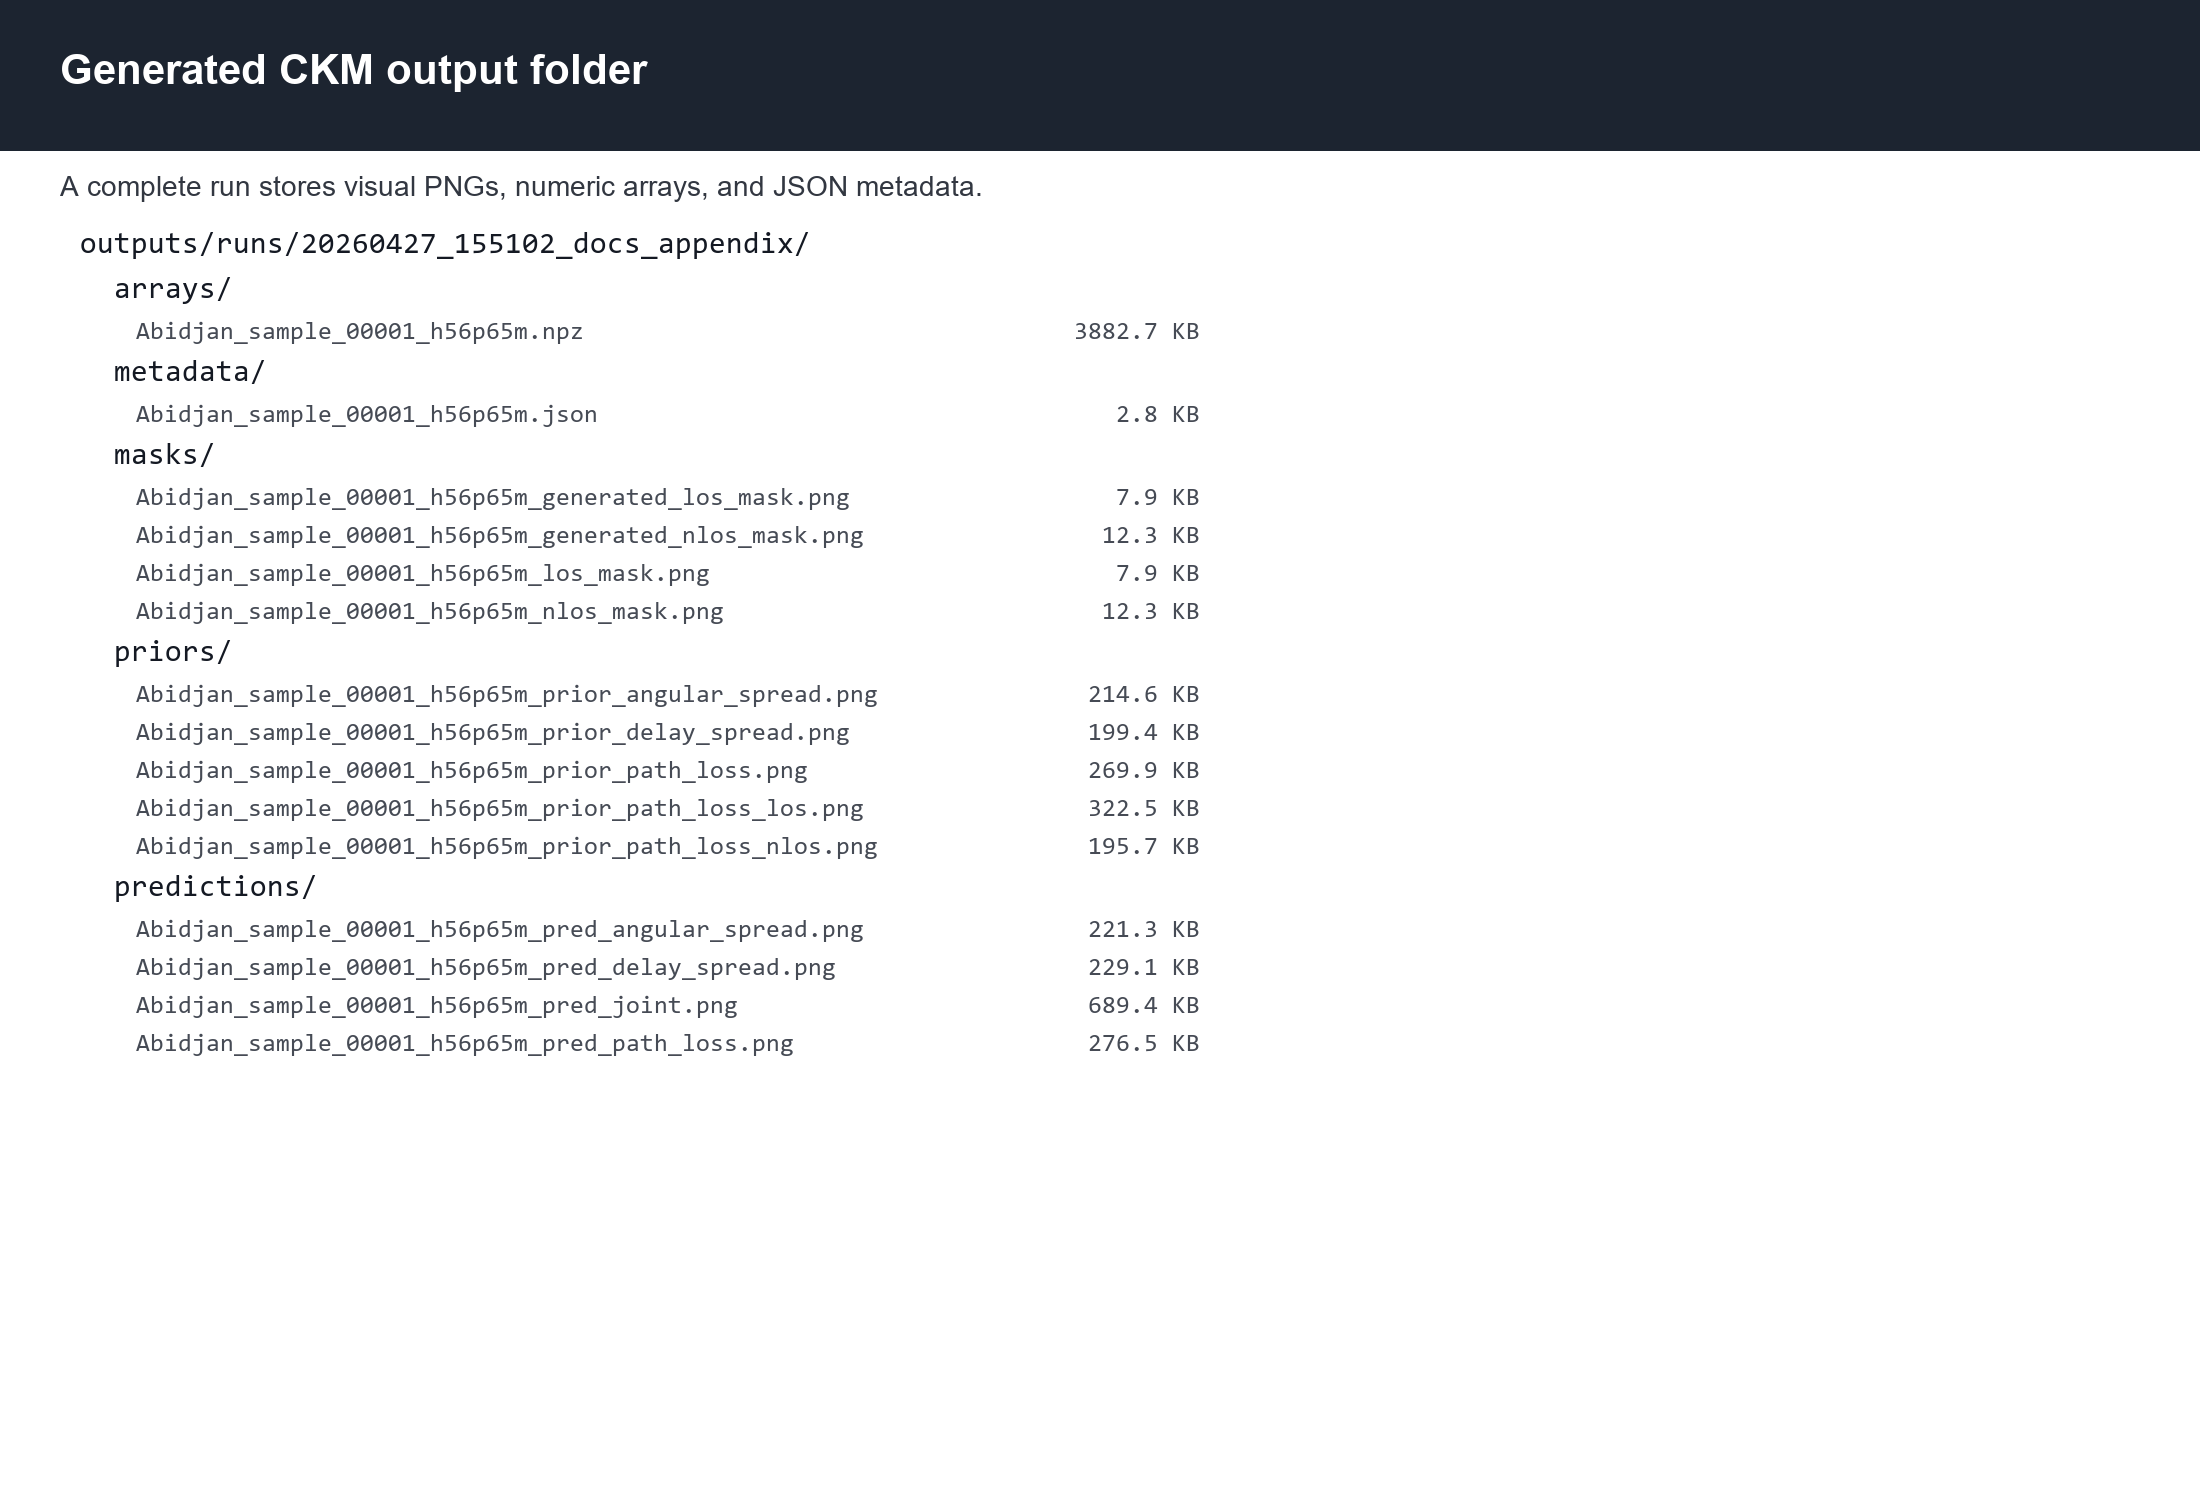
\includegraphics[width=\textwidth,height=0.72\textheight,keepaspectratio]{img/thesis_figures/ckm_generator/ckm_generator_output_tree.png}
\caption{Generated output folder for one CKM Generator run. The run contains
binary masks, prior maps, prediction maps, a compressed numerical archive, and
a JSON metadata file.}
\label{fig:ckm_generator_output_tree}
\end{figure}

\begin{figure}[H]
\centering
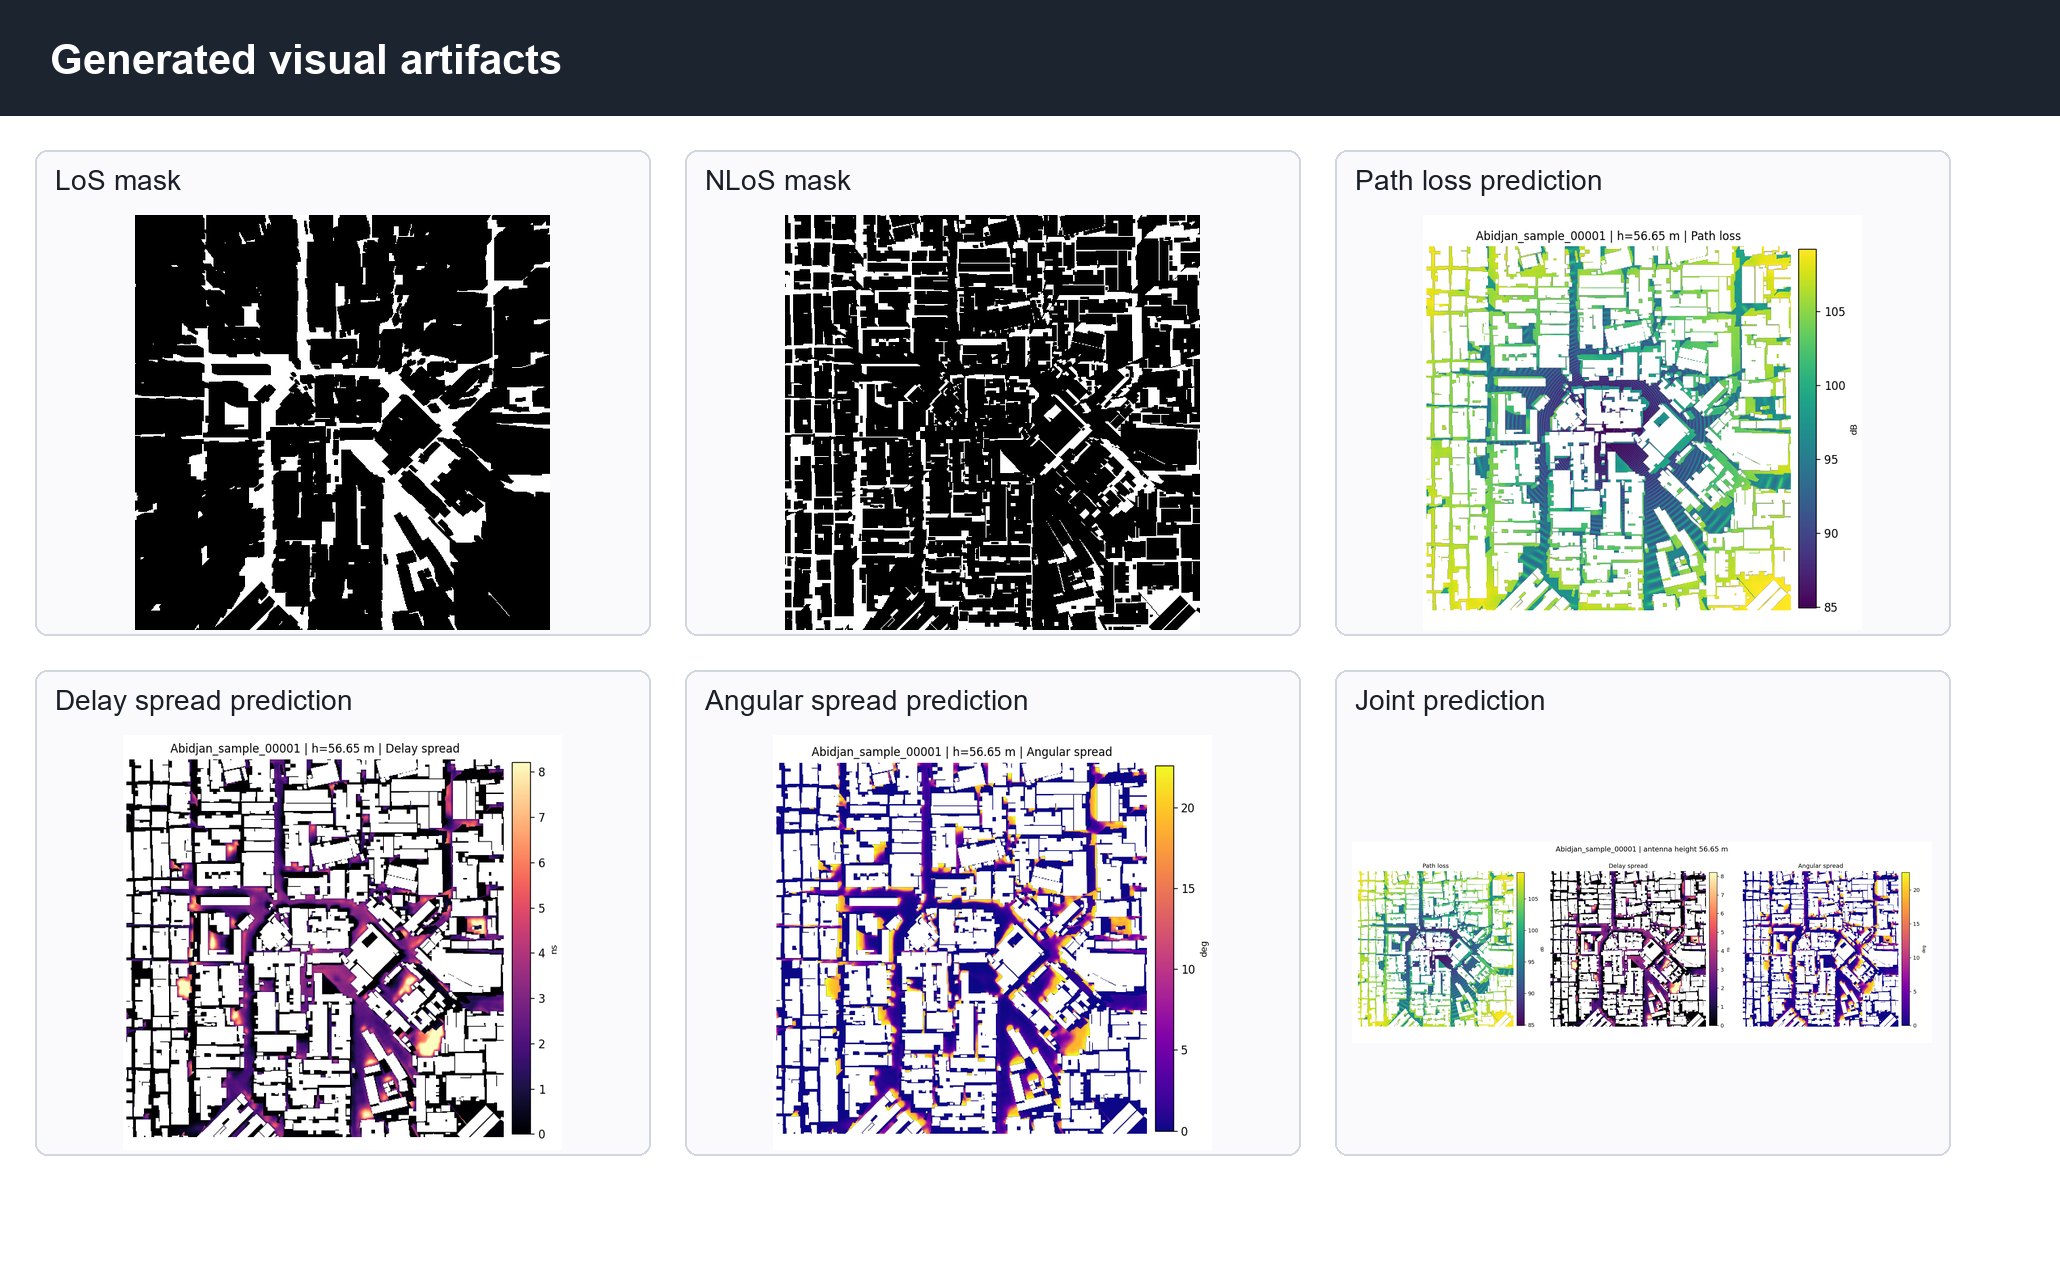
\includegraphics[width=\textwidth,height=0.72\textheight,keepaspectratio]{img/thesis_figures/ckm_generator/ckm_generator_output_visuals.png}
\caption{Visual outputs generated for the same sample: LoS/NLoS masks and the
three Try~80 prediction products, together with the saved joint prediction
panel.}
\label{fig:ckm_generator_output_visuals}
\end{figure}

\begin{figure}[H]
\centering
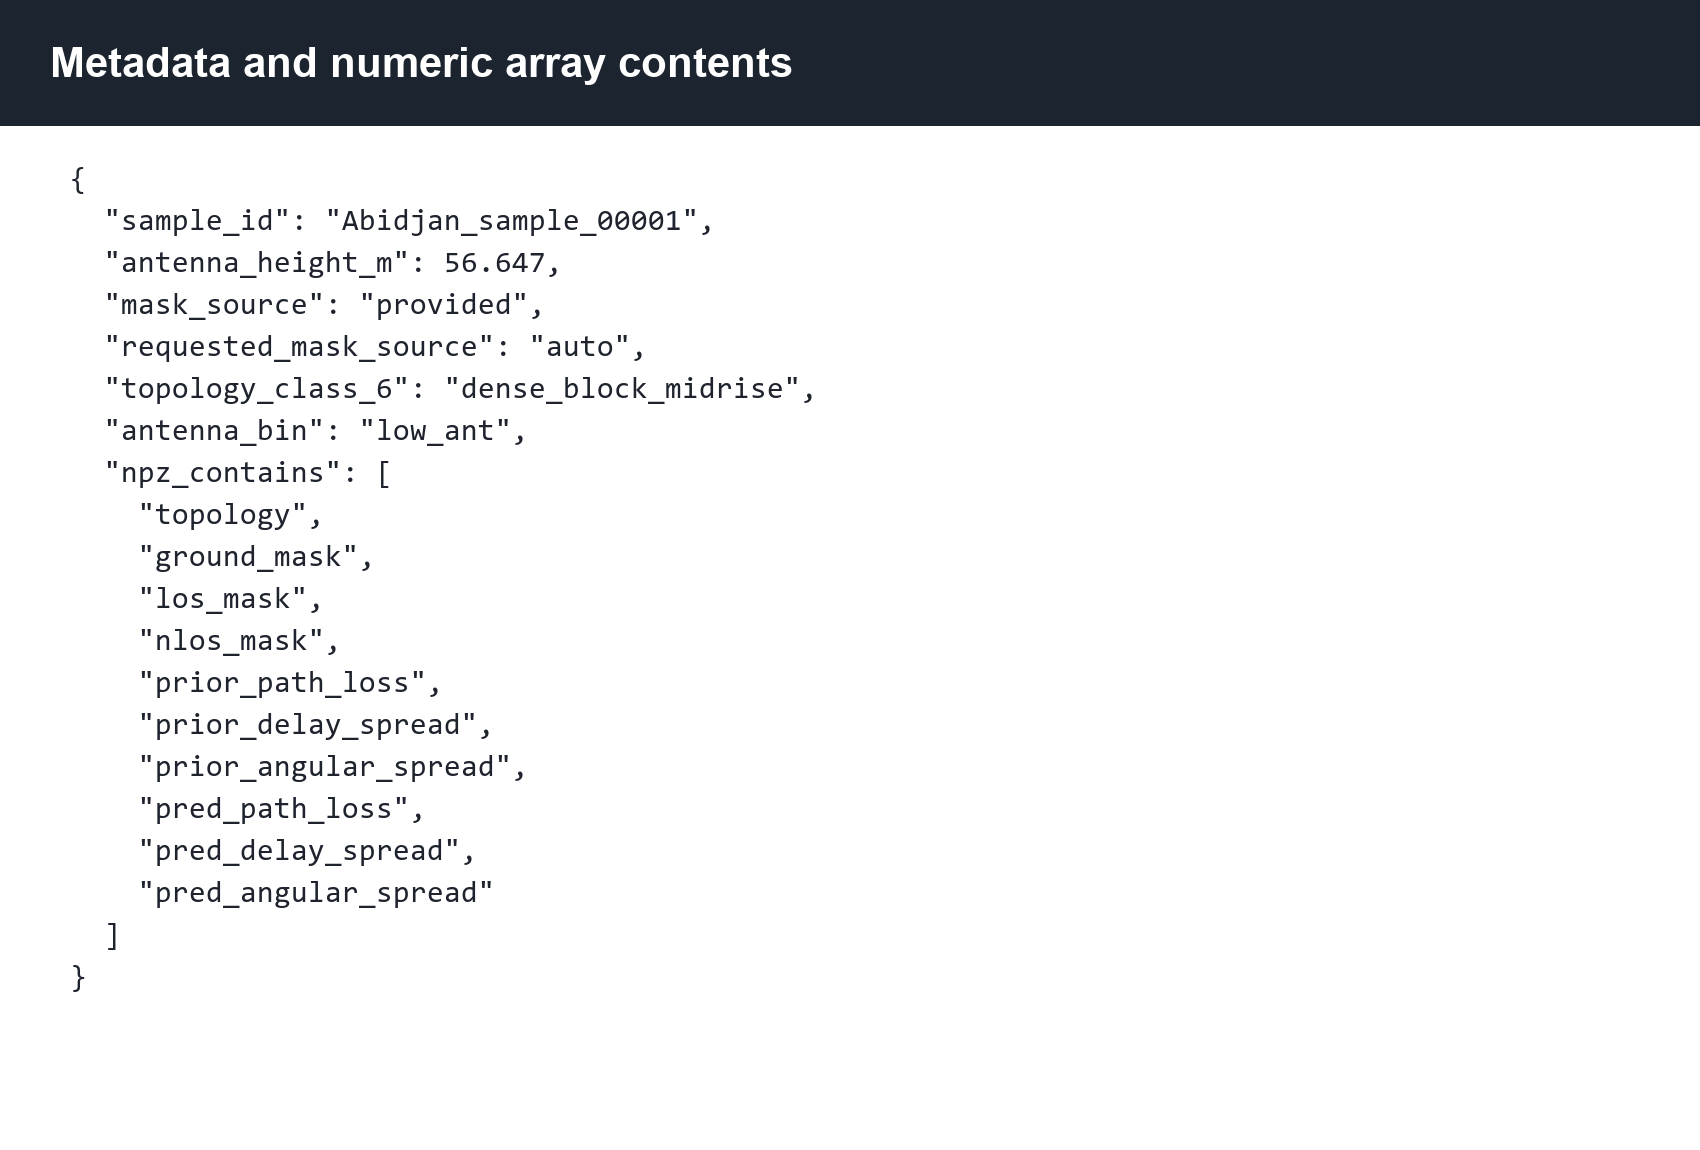
\includegraphics[width=\textwidth,height=0.64\textheight,keepaspectratio]{img/thesis_figures/ckm_generator/ckm_generator_output_metadata.png}
\caption{Example metadata and numerical-array contents for a generated sample.
The metadata records provenance and the resolved mask policy, while the
\texttt{.npz} archive keeps the actual \(513\times513\) numeric maps.}
\label{fig:ckm_generator_output_metadata}
\end{figure}

PNG files are visual inspection products. The authoritative numerical output
is the compressed NumPy archive in \texttt{arrays/}. It stores all arrays on the
final \(513\times513\) grid. Important keys include:
\texttt{topology}, \texttt{ground\_mask}, \texttt{los\_mask},
\texttt{nlos\_mask}, \texttt{generated\_los\_mask},
\texttt{generated\_nlos\_mask}, \texttt{reference\_los\_mask} when available,
\texttt{prior\_path\_loss}, \texttt{prior\_path\_loss\_los},
\texttt{prior\_path\_loss\_nlos}, \texttt{prior\_delay\_spread},
\texttt{prior\_angular\_spread}, \texttt{pred\_path\_loss},
\texttt{pred\_delay\_spread}, and \texttt{pred\_angular\_spread}.

The JSON metadata stores provenance and bookkeeping: sample id, antenna height,
source file, checkpoint path, requested and resolved mask source, topology
class, antenna bin, mask comparison statistics when a reference mask exists,
and the paths of all generated files.

\section{Performance controls}

CUDA is the preferred runtime when available. The app and CLI can also use CPU
or DirectML. The model batch size can increase throughput on GPUs with enough
VRAM, while keeping batch size 1 remains the safest option on smaller cards.

CUDA mixed precision uses PyTorch autocast. On ten exported HDF5 samples,
timing only model inference on the local RTX 3050 Ti Laptop GPU, full fp32 took
approximately \SIrange{6.94}{6.99}{s}, while mixed precision took
\SIrange{5.46}{5.61}{s}. The speedup was about \(1.25\times\). The RMSE
between mixed precision and fp32 predictions was \SI{0.0016}{dB} for path loss,
\SI{0.0034}{ns} for delay spread, and \SI{0.0030}{\degree} for angular spread,
which is negligible compared with the validation RMSE scale of the model.

For batch export, disabling \texttt{Save visual map PNGs} avoids Matplotlib
rendering and keeps only numeric arrays, masks, and metadata. Disabling
\texttt{Run Try 80 model} is useful when the goal is only to validate
topologies, masks, and prior generation.

\chapter{Final-Result Placeholder}

The final Try 80 checkpoint is not yet frozen. Therefore, the validation values
reported in the main chapters must be replaced by final test-split results
before submission. The thesis should keep the current wording until that
evaluation is complete: Try 80 validation results are training diagnostics, not
final scientific claims.
